\documentclass[12pt,hidelinks]{book}
\usepackage{tabularx,titlesec}
\usepackage{graphicx,color,fancyhdr,microtype}
\usepackage{booktabs,enumerate}
\usepackage{framed}
\usepackage{amsmath,amssymb,nth,mathtools,commath,nicefrac,siunitx,bigints,subcaption}
\usepackage{csquotes}

\usepackage[CJKbookmarks]{hyperref}
\hypersetup{
    colorlinks=false,
    %linkcolor=blue,
    %filecolor=magenta,      
    %urlcolor=cyan,
    %pdftitle={Overleaf Example},
    %pdfpagemode=FullScreen,
    }
    
\usepackage[a4paper,top=2.5cm,left=2cm,right=2cm]{geometry}
\usepackage{caption,subcaption} % use "subfigure"

\usepackage{xfrac} % use slanted fraction

\usepackage{physics} % to use bra, ket

\usepackage[utf8]{inputenc} % tell latex it's under utf8

\pagestyle{fancy}
\lfoot{
\includegraphics[scale=.05]{wise_logo_2016.pdf}}
\rfoot{
\includegraphics[scale=.4]{fine_cornell_logo_red_cmyk.eps}}

% bibliography
\usepackage[
	backend=bibtex,
	bibstyle=phys,
	citestyle=numeric-comp,
	articletitle=true,
	biblabel=brackets,
	sorting=none
	]{biblatex}
\addbibresource{reference.bib}

\newcommand*{\Exp}{\mathrm{e}}
\newcommand{\sgn}{\operatorname{sgn}}
\DeclarePairedDelimiter\floor{\lfloor}{\rfloor}
\newcommand{\pvec}[1]{\vec{#1}\mkern2mu\vphantom{#1}}

% Line break if equations are too long
\allowdisplaybreaks[1]

% Differential "d" in the integral. It needs amsmath
\newcommand*\diff{\mathop{}\!\mathrm{d}}
\newcommand*\Diff[1]{\mathop{}\!\mathrm{d^#1}}

\usepackage[version=3]{mhchem}

% MATLAB code
\usepackage{listings,lstautogobble,verbatim}
\definecolor{mygreen}{RGB}{28,172,0} % color values Red, Green, Blue
\definecolor{mylilas}{RGB}{170,55,241}
\definecolor{codebg}{RGB}{237,245,207}
\lstset{language=matlab,
	backgroundcolor=\color{codebg},
    basicstyle=\footnotesize,
    breaklines=true,%
    morekeywords={matlab2tikz},
    keywordstyle=\color{blue},
    morekeywords=[2]{1}, keywordstyle=[2]{\color{black}},
    identifierstyle=\color{black},
    stringstyle=\color{mylilas},
    commentstyle=\color{mygreen},
    showstringspaces=false,%without this there will be a symbol in the places where there is a space
    numbers=left,%
    numberstyle={\tiny \color{black}},% size of the numbers
    numbersep=9pt, % this defines how far the numbers are from the text
    emph=[1]{for,end,break},emphstyle=[1]\color{red}, %some words to emphasise
    autogobble=true,
}

\mathchardef\mhyphen="2D % use hyphen in the math mode; "2D is the ASDII

\title{Solver Guide for the MATLAB solid-core-fiber pulse propagation}
\author{Yi-Hao Chen\\Applied and Engineering Physics, Cornell University}
\date{\today}

\begin{document}
\maketitle
\tableofcontents
\newpage

\chapter{Overview}
\section{Mathematical background}
This package aims to solve the multimode unidirectional pulse propagation equation (MM-UPPE) in a solid-core fiber:
\begin{align}
\partial_zA_p(z,\Omega)& =i\left[\beta_p(\omega)-\left(\beta_{(0)}+\beta_{(1)}\Omega\right)\right]A_p(z,\Omega)+g_p(z,\Omega)A_p(z,\Omega) \nonumber \\
& \hspace{1em}+i\sum_{\ell}Q_{p\ell}A_{\ell}(z,\Omega) \nonumber \\
& \hspace{1em}+\frac{i\omega}{4}\epsilon_0^2n_{\text{eff}}^2cn_2\sum_{\ell mn}\Bigg\{\left(1-f_R\right)Q^K_{p\ell mn}\mathfrak{F}[A_{\ell}A_mA_n^{\ast}] \nonumber \\
& \hspace{11em}
+f_R\bigg\{f_aQ^{R_a}_{p\ell mn}\mathfrak{F}\left[A_{\ell}\left[h_a\ast\left(A_mA_n^{\ast}\right)\right]\right]+ \nonumber \\
& \hspace{14.2em} f_bQ^{R_b}_{p\ell mn}\mathfrak{F}\left[A_{\ell}\left[h_b\ast\left(A_mA_n^{\ast}\right)\right]\right]\bigg\}\Bigg\}, \label{eq:solid_core_UPPE}
\end{align}
which includes dispersion, as well as instantaneous electronic and delayed Raman nonlinearities. $A_p(z,t)$ is the electric field (\si{\sqrt{W}}) of mode $p$, whose Fourier Transform is $A_p(z,\Omega)=\mathfrak{F}[A_p(z,T)]$. The Fourier Transform is applied with respect to angular frequency $\Omega=\omega-\omega_0$, where $\omega_0$ is the center angular frequency of the numerical frequency window required to cover the investigated physical phenomena. $\beta_p$ is the propagation constant of the mode $p$. $\beta_{(0)}$ and $\beta_{(1)}$ are to reduce the propagating global-phase increment to facilitate simulations, $\beta_{(1)}$ is the inverse group velocity of the moving frame, which introduces the delayed time $T=t-\beta_{(1)}z$. $g_p(z,\Omega)$ is the gain (or loss), $n_2$ is the nonlinear refractive index (\si{\m^2/\watt}; refractive index change from nonlinearity $\triangle n=n_2I$ where $I$ is the light intensity), $c$ is the speed of light; $f_R$ is the Raman fraction representing the contribution of the Raman response of all nonlinearities where $f_a$ and $f_b$ are Raman fractions of the total Raman response for isotropic and anisotropic Raman responses, respectively ($f_a+f_b=1$); $h'_a$ and $h'_b$ are isotropic and anisotropic Raman response functions; $p$, $\ell$, $m$, and $n$ the eigenmode indices. $Q^K$, $Q^{R_a}$, and $Q^{R_b}$ are overlap integrals:
\begin{subequations}
\begin{align}
Q^K_{p\ell mn} & =\frac{2}{3}Q^{R_a}_{p\ell mn}+\frac{1}{3}Q^k_{p\ell mn}\qquad,Q^k_{p\ell mn}=\frac{\int\left(\vec{F}_p^{\ast}\cdot\vec{F}_n^{\ast}\right)\left(\vec{F}_{\ell}\cdot\vec{F}_m\right)\diff x\diff y}{N_pN_{\ell}N_mN_n} \label{eq:QK} \\
Q^{R_a}_{p\ell mn} & =\frac{\int\left(\vec{F}_p^{\ast}\cdot\vec{F}_{\ell}\right)\left(\vec{F}_m\cdot\vec{F}_n^{\ast}\right)\diff x\diff y}{N_pN_{\ell}N_mN_n} \label{eq:QRa} \\
Q^{R_b}_{p\ell mn} & =\frac{1}{2}\left[\frac{\int\left(\vec{F}_p^{\ast}\cdot\vec{F}_m\right)\left(\vec{F}_{\ell}\cdot\vec{F}_n^{\ast}\right)\diff x\diff y}{N_pN_{\ell}N_mN_n}+Q^k_{p\ell mn}\right]=\frac{1}{2}\left(Q^{r_b}_{p\ell mn}+Q^k_{p\ell mn}\right), \label{eq:QRb}
\end{align}
\label{eq:Q}
\end{subequations}
where $\vec{F}_p$ is the $p$-th spatial eigenmode, $n_{\text{eff}}$ and $n_{i,\text{eff}}$ in each $N_i$ ($i\in\{p,\ell,m,n\}$) is often taken as the refractive index of silica such that 
\begin{equation}
\frac{\epsilon_0^2n_{\text{eff}}^2c^2}{N_pN_{\ell}N_mN_n}=4.
\label{eq:Q_NNNN_relation}
\end{equation}

With Eq.~(\ref{eq:Q_NNNN_relation}), Eq.~(\ref{eq:solid_core_UPPE}) is simplified to
\begin{align}
\partial_zA_p(z,\Omega)& =i\left[\beta_p(\omega)-\left(\beta_{(0)}+\beta_{(1)}\Omega\right)\right]A_p(z,\Omega)+g_p(z,\Omega)A_p(z,\Omega) \nonumber \\
& \hspace{1em}+i\sum_{\ell}Q_{p\ell}A_{\ell}(z,\Omega) \nonumber \\
& \hspace{1em}+\frac{i\omega n_2}{c}\sum_{\ell mn}\Bigg\{\left(1-f_R\right)S^K_{p\ell mn}\mathfrak{F}[A_{\ell}A_mA_n^{\ast}]+ \nonumber \\
& \hspace{9.5em}
f_R\bigg\{f_aS^{R_a}_{p\ell mn}\mathfrak{F}\left[A_{\ell}\left[h_a\ast\left(A_mA_n^{\ast}\right)\right]\right]+ \nonumber \\
& \hspace{11.5em} f_bS^{R_b}_{p\ell mn}\mathfrak{F}\left[A_{\ell}\left[h_b\ast\left(A_mA_n^{\ast}\right)\right]\right]\bigg\}\Bigg\} , \label{eq:solid_core_UPPE_S}
\end{align}
with modified overlap integrals:
\begin{subequations}
\begin{align}
S^K_{p\ell mn} & =\frac{2}{3}S^{R_a}_{p\ell mn}+\frac{1}{3}S^k_{p\ell mn}\qquad,S^k_{p\ell mn}=\int\left(\vec{F}_p^{\ast}\cdot\vec{F}_n^{\ast}\right)\left(\vec{F}_{\ell}\cdot\vec{F}_m\right)\diff x\diff y \label{eq:SK} \\
S^{R_a}_{p\ell mn} & =\int\left(\vec{F}_p^{\ast}\cdot\vec{F}_{\ell}\right)\left(\vec{F}_m\cdot\vec{F}_n^{\ast}\right)\diff x\diff y \label{eq:SRa} \\
S^{R_b}_{p\ell mn} & =\frac{1}{2}\left[\int\left(\vec{F}_p^{\ast}\cdot\vec{F}_m\right)\left(\vec{F}_{\ell}\cdot\vec{F}_n^{\ast}\right)\diff x\diff y+S^k_{p\ell mn}\right]=\frac{1}{2}\left(S^{r_b}_{p\ell mn}+S^k_{p\ell mn}\right). \label{eq:SRb}
\end{align}
\label{eq:S}
\end{subequations}

In silica, it is sometimes overkill to run with UPPE due to mostly narrowband scenarios. In this case, $\beta(\omega)$ is obtained from its Taylor-series coefficients $\beta_{(0)}+\beta_{(1)}\Omega+\frac{\beta_2}{2}\Omega^2+\frac{\beta_3}{3!}\Omega^3+\cdots$, which is, in fact, equivalent to a more-commonly-used GMMNLSE.

It is worth noting that the field $A_p$ is defined as
\begin{align}
\vec{\mathbb{E}}(\vec{x},t) & =\frac{1}{2}\left[\vec{\mathcal{E}}(\vec{x},t)+\text{c.c.}\right]\quad,\vec{\mathcal{E}}\text{ is the analytic signal of }\vec{\mathbb{E}} \nonumber \\
& =\sum_p\int\diff\omega\frac{1}{2}\left\{\frac{\vec{F}_p(x,y,\omega)}{N_p(\omega)}A_p(z,\omega)\Exp^{i\left[\beta_p(\omega)z-\omega t\right]}+\text{c.c.}\right\}.
\label{eq:Ext}
\end{align}
This makes MATLAB ``ifft'' become the Fourier Transform and ``fft'' become the \emph{inverse} Fourier Transform. The convolution theorem also becomes different with different conventions. In our package, we follow this convention [Eq.~(\ref{eq:Ext})]. For example, to see the spectrum, please use
\begin{lstlisting}[language=MATLAB]
c = 299792.458; % nm/ps
wavelength = c./f; % nm
Nt = size(field,1);
dt = t(2)-t(1); % ps
factor_correct_unit = (Nt*dt)^2/1e3; % to make the spectrum of the correct unit "nJ/THz"
                                    % "/1e3" is to make pJ into nJ
spectrum = abs(fftshift(ifft(field),1)).^2*factor_correct_unit; % in frequency domain
\end{lstlisting}
Use ``fftshift'' to shift the spectrum from small frequency to large frequency. Note that it is not ``ifftshift''. They differ when the number of points is odd. To understand this, think about what the first data point is in ``ifft(field):'' it is the zero-frequency component, so we need to use ``fftshift'' with the frequency defining as
\begin{lstlisting}[language=MATLAB]
f = f0+(-Nt/2:Nt/2-1)'/(Nt*dt); % THz
\end{lstlisting}

Check the supplements of our femtosecond-LWIR generation \cite{Chen2023} and \cite{Chen2024} for details. We forgot to add this information in our JOSAB's multimode-gain paper \cite{Chen2023a}.

\section{High-level understanding of this package}
This package is designed for both single-spatial(transverse) mode or multi-spatial modes. Not only scalar but also polarized fields can be simulated, as well as Raman scattering and the gain. The package exhibits an adaptive control of the step size, except for situations with amplified stimulated emission (ASE). In addition to CPU, highly parallelized cuda computation with a Nvidia GPU is implemented, which is strongly recommended for running with multimodes. In single-mode simulations, for sampling numbers less than approximately $2^{25}$, they can still run faster with CPU than with GPU. The package uses ``RK4IP'' (Runge-Kutta in the interaction picture) for single mode \cite{Heidt2009,Balac2013} and ``MPA'' (Massively Parallel Algorithm) for multimode \cite{Wright2018}.

The fastest way to learn how to use this code is to start with the example codes in the package.

\chapter{Before I go deeply into details}
\section{Introduction}
This document describes how to use the GMMNLSE\_propagate() MATLAB function.

\centerline{\rule{13cm}{0.4pt}}
Below is how to call this function in general.
\begin{lstlisting}[language=MATLAB]
prop_output = GMMNLSE_propagate(fiber, ...
                                initial_condition, ...
                                sim[, ...
                                gain_rate_eqn])
\end{lstlisting}

\begin{description}
\item[prop\_output]\mbox{}\\
It contains the information of the output field after propagating through the fiber, such as the field amplitudes and the positions of each saved field, etc.

\item[fiber]\mbox{}\\
It contains the information of the fiber, such as $\beta_2$, $S^R$, and the MFD, etc.

\item[initial\_condition]\mbox{}\\
It contains the information of the input.\\
Typically it's the input field amplitude. If you run it not only with the rate-equation gain model but considering ASE, it also contains the forward ASE at the input and backward ASE at the output.

\begin{figure}[h!]
\centering
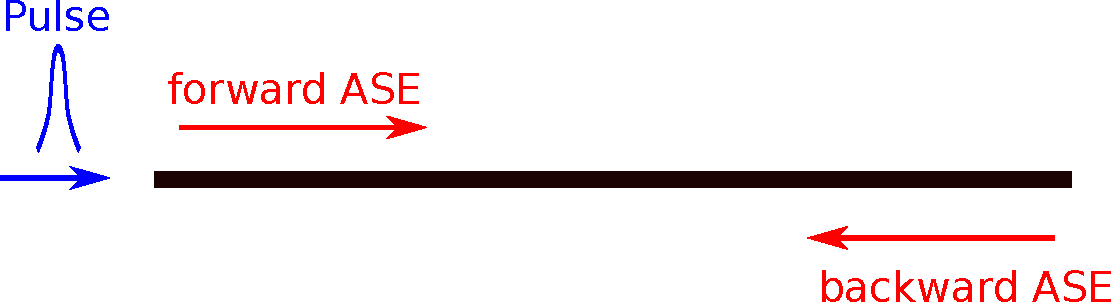
\includegraphics[height=50pt]{initial_condition.pdf}
\caption{Initial conditions}
\label{fig:initial_condition}
\end{figure}

\item[sim]\mbox{}\\
It contains a multitude of information about the simulation, such as the algorithm to use, if running with an adaptive-step method, and the center wavelength, etc.

\item[[gain\_rate\_eqn]]\mbox{}\\
This is required only for the rate-equation gain model.\\
It contains the information required for the rate-equation gain model, such as the pump power, the doped ion density, etc.

\end{description}

\chapter{Input arguments}

Below, I use $N_t$ as the number of time/frequency sampling points, $N_m$ as the number of modes, and $N_{sm}$ as the number of spatial modes. If there is no polarized mode, $N_m=N_{sm}$; otherwise, $N_m=2N_{sm}$.

I recommend to use the information below as a reference guide if you're confused. Start with an example script is always better than reading this first. I have provided some example scripts in Chap.\ref{chap:example}.

Some parameters are required only when you enable some settings. Below I labelled in blue the parameters required all the time.

\section{fiber}
\begin{description}
\item[\color{blue}betas]\mbox{}\\
Typically, this is the variable that saves the $\beta_0, \beta_1, \beta_2\ldots$. It's has the unit of \si{ps^n/m}.

It's a column vector of
\begin{equation}
\begin{bmatrix}
\beta_0 \\ \beta_1 \\ \beta_2 \\ \beta_3 \\ \vdots
\end{bmatrix}
\end{equation}
if this is a single-mode simulation.

For multimode, it becomes
\begin{equation}
\begin{bmatrix}
\beta_{0|1} & \beta_{0|2} & \cdots \\ \beta_{1|1} & \beta_{1|2} & \cdots \\ \beta_{2|1} & \beta_{2|2} & \cdots \\ \beta_{3|1} & \beta_{3|2} & \cdots \\ \vdots & \vdots & \ddots
\end{bmatrix},
\end{equation}
where $\beta_{i|m}$ is the $\beta_i$ for the $m$-th mode.

Besides the narrowband Taylor series expansion of $\beta(\omega)$, I've also implemented the broadband version whose {\bfseries betas} are column vectors of $\beta(\omega)$, that is, it becomes
\begin{equation}
\begin{bmatrix}
\beta_{\cdot|1} & \beta_{\cdot|2} & \cdots
\end{bmatrix},
\end{equation}
where each $\beta_{\cdot|m}$ is a column vector of the propagation constant of the $m$-th mode. It's a function of frequency, with an order from small to large. If the simulation is run with $N_t$ time/frequency points, this $\beta_{\cdot|m}$ should have the length of $N_t$ as well.

\item[\color{blue}n2]\mbox{}\\
It's the nonlinear coefficient of the fiber. By default, GMMNLSE\_propagate() uses \SI{2.3e-20}{m^2/W} assuming we use a silica fiber around \SI{1}{\um} if fiber.n2 is left empty.

\item[\color{blue}SR]\mbox{}\\
It's the overlap integral $S^R$ in scalar GMMNLSE. It's loaded in a dimension of $N_{sm}^4$.

For scalar GMMNLSE, $S^K$ is $S^R$ if the field is linearly polarized or $\frac{2}{3}S^R$ is it's circularly polarized. The unit is \si{m^{-2}}.

For polarized fields, their $S^R$ and $S^K$ can be calculated from the scalar $S^R$. This will be done by GMMNLSE\_propagate() automatically if ``sim.scalar=false.'' For details, check Chap.\ref{chap:polarization}.

\item[\color{blue}L0]\mbox{}\\
This is the fiber length. The unit is meter.

\item[\color{blue}fiber\_type]\mbox{}\\
This specifies the material of the fiber. It's 'silica' by default. It's used only for specifying which Raman model to use. It's either 'silica', 'chalcogenide', or 'ZBLAN'.
\end{description}

\centerline{\rule{13cm}{0.4pt}}
If we use the Gaussian-gain model, the following parameters are required.
\begin{description}
\item[dB\_gain]\mbox{}\\
The small-signal gain amplification of the pulse energy in dB. This is used to calculate the gain\_coeff  (default to 30).

\item[gain\_coeff]\mbox{}\\
This is the small-signal gain coefficient, the $g$ in
\begin{equation}
A(z)=\Exp^{\sfrac{gz}{2}}A(0).
\end{equation}
It's a scalar with the unit of \si{m^{-1}}.

\item[gain\_fwhm]\mbox{}\\
This is the gain bandwidth. A typical number for \ce{Yb}-doped gain fibers is \SI{40}{\nm}. This parameter has the unit of \si{meter}.

\item[gain\_doped\_diameter]\mbox{}\\
The diameter of the doped core to compute the overlap integral between mode fields and the doped core and accurately find their gain.

\item[saturation\_intensity]\mbox{}\\
This is for multimode simulations. It has the unit of \si{J/m^2}.

\item[saturation\_energy]\mbox{}\\
This is for single-mode simulations. It has the unit of \si{nJ}.
\end{description}

\section{initial\_condition}
\begin{description}
\item[\color{blue}dt]\mbox{}\\
This is the time sampling step $\triangle t$ with a unit of \si{\ps}.

\item[\color{blue}fields]\mbox{}\\
This is the input field amplitude under the time domain. It has the unit of \si{\sqrt{W}}. Its size is $N_t\cross N_m$.

If its size is $N_t\cross N_m\cross N_z$, only the last $N_z$ is taken as the input field.
\end{description}

\centerline{\rule{13cm}{0.4pt}}
The two parameters above are required all the time.

If we run the simulation with ASE (and also of course with the rate-equantion gain model), two extra parameters are required. Typically they are both all-zero $N_t\cross N_m$ column vectors.

\begin{description}
\item[Power.ASE.forward]\mbox{}\\
This is the forward ASE at the input ($z=0$). Its array size is the same ``fields'' above.

\item[Power.ASE.backward]\mbox{}\\
This is the backward ASE at the output ($z=L_0$) because backward ASE starts from the output end of the fiber.
\end{description}

\section{sim}
Below are the most basic parameters for a simualtion.
\begin{description}
\item[betas]\mbox{}\\
In UPPE, we not only create a moving frame that follows the pulse with the inverse velocity $\beta_{(1)}$ but extract out the reference propagation constant $\beta_{(0)}$. The benefit of extracting $\beta_{(0)}$ is that it reduces the rate of global phase increment such that the simulation can run with a larger step. This is similar to the limitation of multimode simulations that different spatial modes have different propagation constants that generate beating. To resolve the multimode beating, the size of the z-step cannot be too large.

This ``betas'' is a $2\cross1$ column vector.
\begin{equation}
\begin{bmatrix}
\beta_{(0)} \\ \beta_{(1)}
\end{bmatrix}
\end{equation}

By default, under the narrowband case where fiber.betas is a column vector of the Taylor series coefficient of $\beta(\omega)$, GMMNLSE\_propagate() uses the \nth{1} mode as the reference, that is, 
\begin{equation}
\begin{bmatrix}
\beta_{(0)} \\ \beta_{(1)}
\end{bmatrix}=
\begin{bmatrix}
\beta_{0|1} \\ \beta_{1|1}
\end{bmatrix}.
\end{equation}

\item[\color{blue}f0]\mbox{}\\
The center frequency (\si{\THz}). It's a scalar.

\item[deltaZ]\mbox{}\\
The z-step size (\si{m}). This is required only for non-adaptive-step method. For an adaptive-step method, this parameter varies during computation; setting it here is meaningless.

This may need to be \SIrange[range-units=single,range-phrase = --]{1}{50}{\um} to account for intermodal beating, even if the nonlinear length is large.

\item[\color{blue}save\_period]\mbox{}\\
The length between saved fields (\si{\m}). If it's zero, it's equaivalent to save\_period=fiber.L0 that saves only the input and output fields.

If the simulation doesn't use an adaptive-step method, be aware that this number needs to be a divisor of the fiber length, fiber.L0; otherwise, GMMNLSE\_propagate() will throw an error. For an adaptive-step method, I have the maximum step size set as the $\frac{1}{10}$ of the save\_period and the position of the saved fields will be chosen as the one that first passes through each saved point.
\end{description}

\subsection{MPA}
Here are the parameters if the simulation uses MPA step method \cite{Wright2018}. All parameters are contained within a ``sim.MPA'' structure.

\begin{description}
\item[MPA.M]\mbox{}\\
This is the parallel extent for MPA. \num{1} is no parallelization. \numrange[range-phrase=--]{5}{20} is recommended; there are strongly diminishing returns after \numrange[range-phrase=--]{5}{10}. \num{10} is recommended.

\item[MPA.n\_tot\_max]\mbox{}\\
The maximum number of iterations for MPA. This doesn't really matter because if the step size is too large, the algorithm will diverge after a few iterations. \num{20} is a typical number for this.

\item[MPA.n\_tot\_min]\mbox{}\\
The minimum number of iterations for MPA. \num{2} is recommended.

\item[MPA.tol]\mbox{}\\
The tolerance of convergence for MPA, which is related to the values of the average NRMSE between consecutive itertaions in MPA at which the step is considered converged. \num{e-6} is recommended.
\end{description}

\subsection{Random linear mode coupling}
Here are the parameters if the simulation uses random mode coupling. All parameters are contained within a ``sim.rmc'' structure. To run with random mode coupling, random-coupling matrices need to be created beforehand by calling
\begin{lstlisting}[language=MATLAB]
save_points=int32(fiber.L0/sim.deltaZ);
sim.rmc.matrices = create_rmc_matrices(fiber,sim,num_modes,save_points);
\end{lstlisting}
``sim.deltaZ'' is required since there is no adaptive step-size control for computations with random mode coupling.

\begin{description}
\item[\color{blue}rmc.model]\mbox{}\\
\begin{tabular}{ll}
false (0) & includes random mode coupling \\
true (1) & don't include random mode coupling
\end{tabular}

\item[rmc.varn]\mbox{}\\
The variations of refractive index of the fiber. It is used to control the strength of random mode coupling.

\item[rmc.stdQ\_polarizedmode]\mbox{}\\
Similar to ``rmc.varn'', it is used control the strength of random polarization-mode coupling.

\item[rmc.lambda0]\mbox{}\\
It lets the code know the wavelength of the eigenmode fields to load for random mode coupling to compute the coupling strengths.

\item[rmc.downsampling\_factor]\mbox{}\\
To compute the couplng strengths among spatial modes, loading mode profiles is required. This downsampling factor determines the downsampled factor after loading to improve the performance of the random-mode-coupling matrices. Since it won't affect the latter nonlinear pulse propagation, I typically just set it to \num{1}.
\end{description}

\subsection{Polarization modes}
Here are the parameters if the simulation includes polarization modes.

\begin{description}
\item[\color{blue}scalar]\mbox{}\\
\begin{tabular}{ll}
false (0) & includes polarization-mode coupling \\
true (1) & don't include polarization-mode coupling
\end{tabular}

If the simulation is solved with ``sim.scalar=true,'' the input field takes only the scalar fields, e.g., 
\[
\begin{bmatrix}
\text{mode 1} & \text{mode 2} & \text{mode 3} & \ldots
\end{bmatrix}.
\]
Otherwise, the input field of each polarized mode needs to be specified in the order of
\[
\begin{bmatrix}
\text{mode 1}_+ & \text{mode 1}_- & \text{mode 2}_+ & \text{mode 2}_- & \ldots
\end{bmatrix},
\]
where (+,-) can be (x,y), (right-handed circular, left-handed circular), or any orthogonally polarized modes.

Based on whether to include polarization-mode coupling, $S^R$ and $S^K$ are automatically calculated to its polarized version by GMMNLSE\_propagate().

\item[\color{blue}ellipticity]\mbox{}\\
The ellipticity of the polarization modes. Please refer to ``Nonlinear Fiber Optics, eq (6.1.18) Agrawal'' for the equations.

\begin{tabular}{lll}
0 & linear polarization & (+,-)=(x,y) \\
1 & circular polarization & (+,-)=(right,left)
\end{tabular}
\end{description}

\subsection{Adaptive-step method}
Here are the parameters if the simulation uses adaptive-step method. All parameters are contained within a ``sim.adaptive\_deltaZ'' structure. The user doesn't need to specify whether to use adaptive-step method or not; the code determines itself. With the adaptive-step method, the initial step size is set to a small \SI{e-6}{\m}.

\begin{description}
\item[adaptive\_deltaZ.threshold]\mbox{}\\
The threshold of the adaptive-step method. It controls the accuracy of the simulation and determines whether to increase or decrease the step size. I typically use $10^{-6}$.

\item[adaptive\_deltaZ.max\_deltaZ]\mbox{}\\
The maximum z-step size (\si{m}) of the adaptive-step method. It's 1/10 the save\_period by default.
\end{description}

\subsection{Algorithm to use}
\begin{description}
\item[\color{blue}gpu\_yes]\mbox{}\\
\begin{tabular}{ll}
true (1) & use GPU \\
false (0) & don't use GPU
\end{tabular}

\item[\color{blue}Raman\_model]\mbox{}\\
\begin{tabular}[t]{ll}
0 & ignore Raman effect \\
1 & Raman model approximated analytically by a single vibrational frequency of molecules\\
& (Ch. 2.3, p.42, Nonlinear Fiber Optics (5th), Agrawal) \\
2 & Raman model including the anisotropic contribution \\
& (``Ch. 2.3, p.43'' and ``Ch. 8.5, p.340,'' Nonlinear Fiber Optics (5th), Agrawal)
\end{tabular}

For more details about anisotropic Raman, please read ``Raman response function for silica fibers,'' by Q. Lin and Govind P. Agrawal (2006). Besides silica, chalcogenide and ZBLAN are also included.

\item[\color{blue}gain\_model]\mbox{}\\
Except for the rate-equation gain model, all the other gain models use a Gaussian gain; thus, the gain\_coeff, gain\_fwhm, and gain saturation intensity or energy need to be specified in ``fiber.''

\begin{tabular}{ll}
0 & no gain \\
1 & Gaussian gain \\
2 & rate-equation gain: see Chap.\ref{chap:rategain} for details
\end{tabular}

\item[\color{blue}pulse\_centering]\mbox{}\\
Because the pulse will evolve in the fiber, it's hard to have the moving frame always move with the same speed as the pulse. As a result, the pulse will go out of the time window and come back from the other side due to the use of periodic assumption of discrete Fourier Transform. The shift in time is saved in ``prop\_output.t\_delay'' so that you don't lose the information

When enabling pulse\_centering, the pulse will be centered to the center of the time window based on the moment of the field intensity ($\abs{A}^2$).

\begin{tabular}{ll}
true (1) & center the pulse according to the time window \\
false (0) & don't center the pulse
\end{tabular}

\item[\color{blue}include\_sponRS]\mbox{}\\
\begin{tabular}{ll}
true (1) & include spontaneous Raman term \\
false (0) & don't include spontaneous Raman term
\end{tabular}

\item[\color{blue}include\_noise]\mbox{}\\
For a Raman or four-wave-mixing process, it's important to include the shot noise to generate a reasonably strong signal. The strength of noise is controlled by ``num\_photon\_noise\_per\_band''.

\begin{tabular}{ll}
true (1) & include photon noise \\
false (0) & don't include the photon noise
\end{tabular}

\item[\color{blue}num\_photon\_noise\_per\_bin]\mbox{}\\
This controls the number of photon noise to include per spectral discretization bin. It's default to \num{1}.

\begin{equation}
P_{\text{noise}}=hf/\left(N\triangle t\right),
\end{equation}
whose relation depends on the convention of Fourier Transform. For convention of the laser field, Fourier Transform is defined as MATLAB's ``ifft,'' which leads to the relation here. With a different convention, the multiplication factor might be different from $1/\left(N\triangle t\right)$.

\item[\color{blue}cuda\_dir\_path]\mbox{}\\
The path to the cuda directory into which ptx files will be compiled and stored. This is ``/GMMNLSE/cuda/.''

\item[gpuDevice.Index]\mbox{}\\
The GPU to use. It's typically 1 if the computer has only one GPU. MATLAB starts the index with 1.
\end{description}

\centerline{\rule{13cm}{0.4pt}}
Here are the parameters for the progress bar used in the simulation. It's useful in general to see how a simulation progresses.

\begin{description}
\item[\color{blue}progress\_bar]\mbox{}\\
\begin{tabular}{ll}
true (1) & show progress bar \\
false (0) & don't show progress bar
\end{tabular}

\item[progress\_bar\_name]\mbox{}\\
The name of the GMMNLSE shown on the progress bar. If not set (no ``sim.progress\_bar\_name''), it uses a default empty string, ''.
\end{description}

\chapter{Output arguments}

\begin{description}
\item[fields]\mbox{}\\
The $N_t\cross N_m\cross N_z$ output fields.

\item[dt]\mbox{}\\
This is the time sampling step $\triangle t$ with a unit of \si{\ps}.

\item[z]\mbox{}\\
This is the positions of each saved field.

\item[deltaZ]\mbox{}\\
The z-step size (\si{\m}).

For an adaptive-step method, this contains the step size at each saved point. You can see how the step size evolves through the propagation with this parameter.

\item[betas]\mbox{}\\
The ``sim.betas,''[$\beta_{(0)};\beta_{(1)}$] , used in this propagation.

\item[t\_delay]\mbox{}\\
The time delay of the pulse at each saved point due to pulse centering.

\item[seconds]\mbox{}\\
The time spent for this simulation.
\end{description}

\section{For rate-equation gain model}
\subsection{Power}
Here saves the pump and ASE power. They are saved in the ``prop\_output.Power'' structure.

\begin{description}
\item[Power.pump.forward]\mbox{}\\
The forward pump power along the fiber. Its size is $1\cross1\cross N_z$.

\item[Power.pump.backward]\mbox{}\\
The backward pump power along the fiber. Its size is $1\cross1\cross N_z$.
\end{description}

\centerline{\rule{13cm}{0.4pt}}
If ASE is considered,

\begin{description}
\item[Power.ASE.forward]\mbox{}\\
The forward ASE power along the fiber. Its size is $N_t\cross N_m\cross N_z$ if run with multimode and $1\cross1\cross N_z$ if run with single mode.

\item[Power.ASE.backward]\mbox{}\\
The backward ASE power along the fiber. Its size is $N_t\cross N_m\cross N_z$ if run with multimode and $1\cross1\cross N_z$ if run with single mode.
\end{description}

\subsection{Others}
If the population inversion, N2, is exported,
\begin{description}
\item[N2]\mbox{}\\
The doped ion density of the upper-state population. Its size is $N_x\cross N_x\cross N_z$ if run with multimode and $1\cross1\cross N_z$ if run with single mode. $N_x$ is the number of cross-sectional spatial sampling.
\end{description}

\centerline{\rule{13cm}{0.4pt}}
The following output occrus only when gain\_rate\_eqn.reuse\_data=true.

\begin{description}
\item[saved\_data]\mbox{}\\
This is used for an oscillator to converge faster. There's no need for a user to read this. It'll be sent to GMMNSLE\_propagate() in the next roundtrip.
\end{description}

\chapter{Polarization modes}
\label{chap:polarization}
If the simulation is solved with ``sim.scalar=true,'' the input field takes only the scalar fields, e.g., 
\[
\begin{bmatrix}
\text{mode 1} & \text{mode 2} & \text{mode 3} & \ldots
\end{bmatrix}.
\]
Otherwise, the input field of each polarized mode needs to be specified in the order of
\[
\begin{bmatrix}
\text{mode 1}_+ & \text{mode 1}_- & \text{mode 2}_+ & \text{mode 2}_- & \ldots
\end{bmatrix},
\]
where (+,-) can be (x,y), (right-handed circular, left-handed circular), or any orthogonally polarized modes.

If the input $\beta$ has a dimension of only the number of spatial modes, $N_{sm}$, I assume there's no significant influence from birefringence; thus, it's expanded into $2N_{sm}$ dimension with each $i$ and $j$ (polarization) modes being degenerate by GMMNLSE\_propagate(). For polarized fields,
\begin{align}
S^R_{plmn} & =\frac{\int\diff x\diff y\Big[\mathbf{F}_p^*\cdot\mathbf{F}_l\Big]\Big[\mathbf{F}_m^*\cdot\mathbf{F}_n\Big]}{\left[\left(\int\diff x\diff y\abs{\mathbf{F}_p}^2\right)\left(\int\diff x\diff y\abs{\mathbf{F}_l}^2\right)\left(\int\diff x\diff y\abs{\mathbf{F}_m}^2\right)\left(\int\diff x\diff y\abs{\mathbf{F}_n}^2\right)\right]^{\sfrac{1}{2}}} \\
S^K_{plmn} & =\frac{2}{3}S^R_{plmn}+\frac{1}{3}\frac{\int\diff x\diff y\Big[\mathbf{F}_p^*\cdot\mathbf{F}_n^*\Big]\Big[\mathbf{F}_m\cdot\mathbf{F}_l\Big]}{\left[\left(\int\diff x\diff y\abs{\mathbf{F}_p}^2\right)\left(\int\diff x\diff y\abs{\mathbf{F}_l}^2\right)\left(\int\diff x\diff y\abs{\mathbf{F}_m}^2\right)\left(\int\diff x\diff y\abs{\mathbf{F}_n}^2\right)\right]^{\sfrac{1}{2}}}\
\end{align}

Therefore, $S^R_{plmn}$ isn't zero as (p,l) and (m,n) both have the same polarization, and we get four possibilities for (p,l,m,n), (0,0,0,0), (0,0,1,1), (1,1,0,0), and (1,1,1,1), with their values directly derived from the scalar $S^R_{plmm}$. For $S^K_{plmn}$, in addition to the permutations of $S^R_{plmn}$, we need to consider those from the fraction above which isn't zero as (p,l,m,n) is (0,0,0,0), (0,1,1,0), (1,0,0,1), and (1,1,1,1). Notice that some of them can add up with $S^R_{plmn}$ while some of them can't, so the value has a prefactor of $1, \frac{2}{3}, \frac{1}{3}$.

The above generalization of the scalar $S^R$ to polarized $S^R, S^K$ needs each $\mathbf{F}_p$ to be either parallel or orthogonal to one another, so (i,j) has to be an orthogonal group in 2D, e.g., $(x,y)$ or $(\sigma_+,\sigma_-)$.

\chapter{Rate-equation gain model}
\label{chap:rategain}
To run with rate-equation gain model, you need to run ``gain\_info()'' first. This precomputes the required information for this model and saves the computational time. For example, it computes the doped ion density based on the absorption and the cladding area. It also loads the multimode spatial profiles for multimode gain evolution.

\centerline{\rule{13cm}{0.4pt}}
Below is the code sequence of how to run the rate-equation gain model:
\begin{lstlisting}[language=MATLAB]
f = ifftshift( (-N/2:N/2-1)/N/dt + sim.f0 ); % in the order of "omegas" in GMMNLSE_propagate()
c = 299792.458; % nm/ps
lambda = c./f; % nm

% First call gain_info():
gain_rate_eqn = gain_info( fiber,sim,gain_rate_eqn,lambda );

% And then send it to GMMNLSE_propagate():
output_field = GMMNLSE_propagate( fiber,input_field,sim,gain_rate_eqn );
\end{lstlisting}

\section{Input arguments}
Most of the important parameters are contained in the gain\_rate\_eqn structure.
Some parameters are used only with multimode simualtions. I labelled in blue those required all the time whether it's single-mode or multimode. I put (SM) if it's only for single-mode simulations and (MM) if it's only for multimode ones.

\subsection{gain\_rate\_eqn}
\subsubsection{\underline{Multimode mode-profile folder}}
\begin{description}
\item[MM\_folder$^{\text{(MM)}}$]\mbox{}\\
A string; where the betas.mat and S\_tensor\_?modes.mat are. This is used only for multimode simulations which need to load their betas and SR values in the mat files from the mode solver.
\end{description}

\subsubsection{\underline{Oscillator info}}
\begin{description}
\item[\color{blue}reuse\_data]\mbox{}\\
True (1) or false (0).

For a ring or linear cavity, the pulse will enter a steady state eventually. If reusing the pump and ASE data from the previous roundtrip, the convergence can be much faster, especially for counterpumping.

\item[\color{blue}linear\_oscillator]\mbox{}\\
True (1) or false (0), about whether the simulation is for a linear oscillator.

For a linear oscillator, there are pulses from both directions simultaneously, which will both contribute to saturating the gain; therefore , the backward-propagating pulses need to be taken into account.

For a linear oscillator, gain\_rate\_eqn.reuse\_data must be ``true'' to consider the backward-propagating pulses. If gain\_rate\_eqn.reuse\_data is ``false'', gain\_info() will correct it to ``true''.

How to use it:
\begin{lstlisting}[language=MATLAB]
% previous_rate_gain_saved_data comes from the GMMNLSE_propagate() output from the previous roundtrip
gain_rate_eqn.saved_data = previous_rate_gain_saved_data;
prop_output = GMMNLSE_propagate(fiber,...
                                input_field,...
                                sim,...
                                gain_rate_eqn);
(next)previous_rate_gain_saved_data = prop_output.saved_data;
\end{lstlisting}
\end{description}

\subsubsection{\underline{Gain-fiber info}}
\begin{description}
\item[\color{blue}core\_diameter]\mbox{}\\
For double-clad fibers, this is where the doped ion is and the pulse propagates in (\si{\um}).

\item[\color{blue}cladding\_diameter]\mbox{}\\
The cladding diameter (\si{\um}).

\item[core\_NA$^{\text{(SM)}}$]\mbox{}\\
The core numerical aperture of the gain fiber. This is used only for single-mode simulations to calculate the MFD and further the overlap factor between the signal pulse and the doped ion. For multimode, the overlap factor is obtained from loaded spatial profiles; therefore, it doesn't need core\_NA.
\end{description}

\subsubsection{\underline{Doped-ion info}}
\begin{description}
\item[\color{blue}absorption\_wavelength\_to\_get\_N\_total]\mbox{}\\
The wavelength specified by the manufacturer which they use to measure the absorption of the gain fiber (\si{\nm}).

\item[\color{blue}absorption\_to\_get\_N\_total]\mbox{}\\
The absorption measured with the wavelength specified above (\si{\dB/m}).

If the pump power is weak such that the upper-state population is negligible ($N_2=0$, and thus $N_1=N_{\text{total}}$), pump power follows
\begin{equation}
P_P(z+\triangle z)=\exp\left(-\frac{A_{\text{core}}}{A_{\text{cladding}}}\sigma_a(\nu_P)N_{\text{total}}(z)\triangle z\right)P_P(z).
\end{equation}
Therefore, the absorption in \si{\decibel/\m} is $\alpha_{\si{\decibel/\m}}=10\log_{10}\left[\exp\left(\frac{A_{\text{core}}}{A_{\text{cladding}}}\sigma_a(\nu_P)N_{\text{total}}(z)\right)\right]$, which leads to the total doped-ion population
\begin{equation}
N_{\text{total}}=\frac{\ln\left(10^{\alpha_{\si{\decibel/\m}}/10}\right)}{\frac{A_{\text{core}}}{A_{\text{cladding}}}\sigma_a(\nu_P)}=\frac{\frac{\alpha_{\si{\decibel/\m}}}{10}\ln\left(10\right)}{\frac{A_{\text{core}}}{A_{\text{cladding}}}\sigma_a(\nu_P)}.
\end{equation}

\item[\color{blue}cross\_section\_filename]\mbox{}\\
The filename of the data of the doped-ion cross section. It contains both the emisson and absorption cross sections.

Currently I have '\textbf{Liekki\ Yb\_AV\_20160530.txt}' and '\textbf{Yb\_Gen\_VIII\_Cross\_Section\ (Nufern).txt}' for Yb and '\textbf{optiwave\ Er.txt}' for Er.

Er data is from \href{https://optiwave.com/resources/applications-resources/optical-system-edfa-basic-concepts/}{the optiwave website}. Nufern (currently bought by Coherent) Yb data is from \href{https://www.coherent.com/resources/application-note/components-and-accessories/specialty-optical-fibers/yb-absorption-emission.pdf}{their spreadsheet}.

\begin{figure}[h!]
\centering
\begin{subfigure}{0.3\textwidth}
\centering
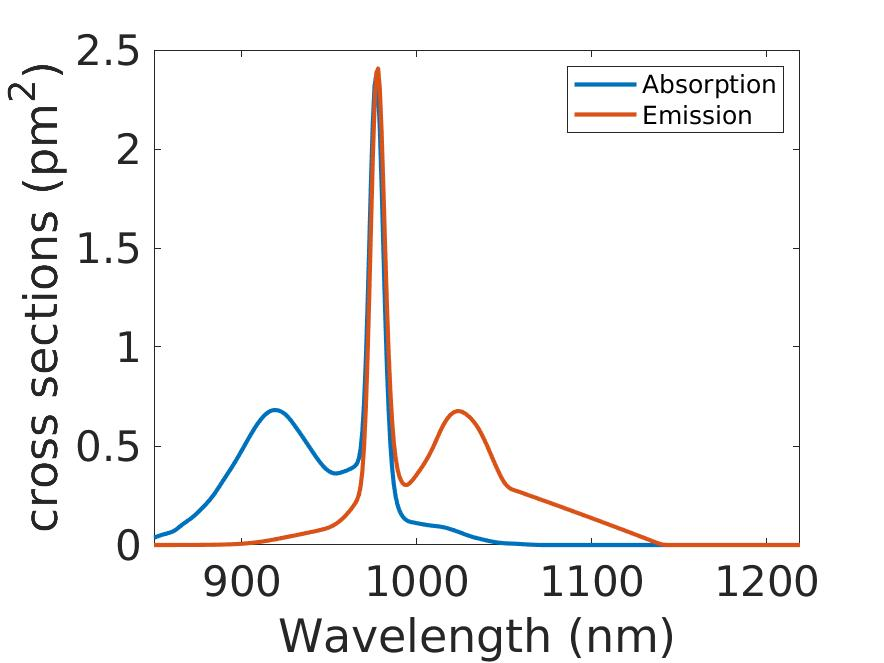
\includegraphics[width=\textwidth]{Yb (Liekki).jpg}
\caption{Yb (Liekki)}
\end{subfigure}
\begin{subfigure}{0.3\textwidth}
\centering
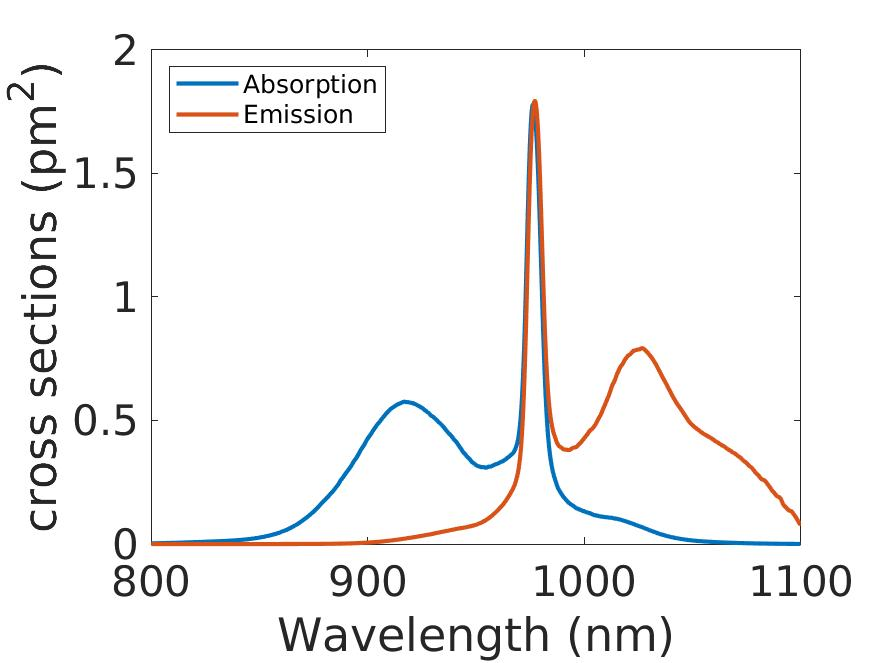
\includegraphics[width=\textwidth]{Yb (Nufern).jpg}
\caption{Yb (Nufern)}
\end{subfigure}
\begin{subfigure}{0.3\textwidth}
\centering
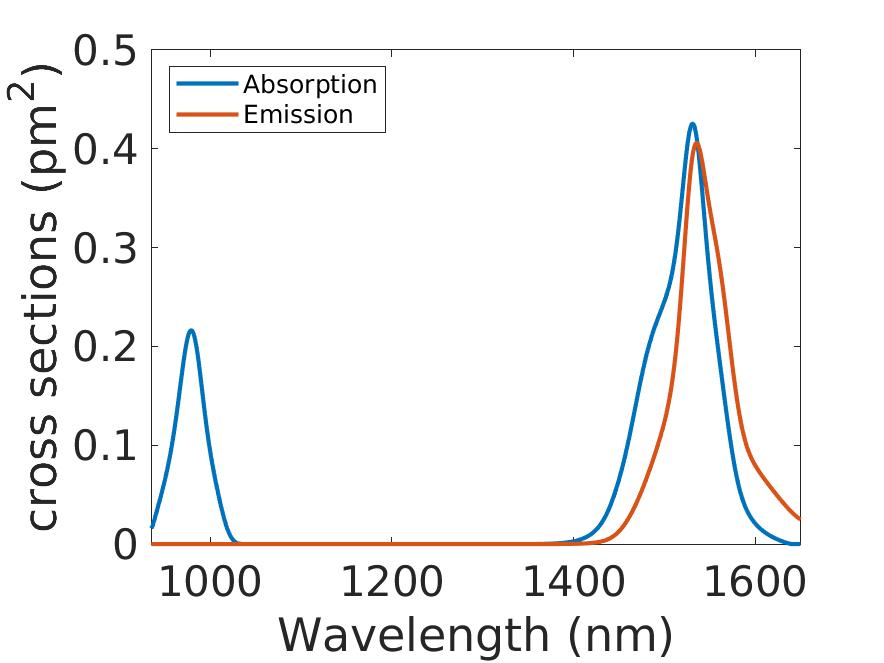
\includegraphics[width=\textwidth]{Er (optiwave).jpg}
\caption{Er (Optiwave)}
\end{subfigure}
\caption{Absorption and emission cross sections.}
\end{figure}
\end{description}

\subsubsection{\underline{Pump info}}
\begin{description}
\item[\color{blue}pump\_wavelength]\mbox{}\\
The pump wavelength (\si{\nm}).

\item[\color{blue}copump\_power]\mbox{}\\
This is the pump sending in from the input end of the fiber (\si{\W}). It co-propagates with the signal pulse. If it's counterpumping, set this to zero.

\item[\color{blue}counterpump\_power]\mbox{}\\
This is the pump sending in from the output end of the fiber (\si{\W}). It counter-propagates with the signal pulse. If it's copumping, set this to zero.
\end{description}

\subsubsection{\underline{Mode profiles}}
If ``mode\_profiles'' is ignored in the input arguments of gain\_info(), it will read the mode profiles from gain\_rate\_eqn.MM\_folder. Some extra operations on these mode profiles are done with the following parameters.

\begin{description}
\item[downsampling\_factor$^{\text{(MM)}}$]\mbox{}\\
This is the factor of downsampling that reduces the size of mode profiles for multimode. Typically the loaded mode profiles from the mode solver is $800\cross800$, so downsampling it down to $100\cross100$, or even smaller, speeds up a simulation a lot. Under this circumstances, gain\_rate\_eqn.downsampling\_factor=8.
\end{description}

\subsubsection{\underline{Computational info}}
\begin{description}
\item[\color{blue}tau]\mbox{}\\
The lifetime of the upper states, which is used in spontaneous emission (\si{s}).

\begin{enumerate}
\item $\text{lifetime of \ce{Yb} in \ce{F_{5/2}} state}=\SI{840}{\us}$ (Paschotta et al., ``Lifetme quenching in Yb-doped fibers'')
\item $\text{lifetime of \ce{Er} in \ce{{^4}I_{13/2}} state}=\SIrange[range-units=single,range-phrase = \mhyphen]{8}{10}{\ms}$
\end{enumerate}

\item[\color{blue}t\_rep]\mbox{}\\
The roundtrip time (1/repetition rate) of the pulse, which is used to calculate the power of the ``signal'' pulse (\si{\s}).

This rate-equation gain model assumes a high repetition rate such that the gain is able to reach a steady state. Therefore, the information of the repetition rate of the pulse is necessary. If the repetition is too low, gain\_info() will throw a warning.
\end{description}

\subsubsection{\underline{ASE info}}
\begin{description}
\item[\color{blue}ignore\_ASE]\mbox{}\\
True (1) or false (0).

\item[\color{blue}sponASE\_spatial\_modes]\mbox{}\\
The number of available spatial modes for ASE.

In principle, the number of spatial modes for ASE should be the same as those for signal fields. However, due to computational simplicity, a smaller number of spatial modes for signal fields might be considered. In such a situation, ASE spatial modes should still be considered to correctly approximate the amount of generated ASE. For example, in large-mode-area fibers, the number of ASE modes can be larger than that of the signal field, where usually, only the fundamental mode is considered for the signal field due to fiber coiling. If this value is left empty like ``[~]'', it is ``length(sim.midx),'' the number of signal spatial modes. I use ``sponASE'' because ASE grows from spontaneous emission. The number of spatial modes manifests itself as more spontaneous emission generated.
\end{description}

\subsubsection{\underline{Algorithm info}}
\begin{description}
\item[\color{blue}export\_N2]\mbox{}\\
True (1) or false (0). Whether to export N2, the ion density of the upper state, or not.

\item[\color{blue}max\_iterations]\mbox{}\\
The maximum number of iterations.

If having iterations is required, you can see that more iterations are needed for a longer fiber to converge. Play around this value to get the result to converge.

\item[\color{blue}tol]\mbox{}\\
The tolerance of this iteration. If the difference of pulse energy or ASE power between the last two results is smaller than this tolerance, it's done.

\item[\color{blue}verbose]\mbox{}\\
Show the information (final pulse energy) during iterations.

\item[memory\_limit]\mbox{}\\
The memory limit for the simulation. This can be found by default. It's important only when gain\_rate\_eqn.reuse\_data=true for an oscillator.

With GPU computing, it is ``sim.gpuDevice.Device.AvailableMemory/2''. Otherwise, it looks for the available RAM for MATLAB and becomes ``$\text{userview.MemUsedMATLAB}/2\cdot 2^{20}$'' for windows. This is supported only under windows and linux, not iOS because I have no experience in iOS. The command between linux and iOS shouldn't differ too much, it's possible to implement it.
\end{description}

\subsection{lambda and mode\_profiles}
\begin{description}
\item[\color{blue}lambda]\mbox{}\\
The wavelengths of the simulation (\si{\nm}). It's ordered as right after taking ``ifft.'' Check the code of how to call gain\_info() at the beginning of this chapter.
\end{description}

\subsubsection{\underline{mode profiles}}
If this isn't specified or left empty, gain\_info() will load mode profiles from gain\_rate\_eqn.MM\_folder.

\begin{description}
\item[mode\_profiles]\mbox{}\\
The eigenmode profiles of field amplitudes. It'll be normalized into the unit of \si{1/\um} in gain\_info().

\item[mode\_profiles\_x]\mbox{}\\
The x-position of mode profiles (\si{\um}). It's an array of length $N_x$.
\end{description}

\section{Output arguments}
Precomputing overlap\_factor, FmFnN, and GammaN is the main reason of running this function before GMMNLSE\_propgate() with the rate-equation gain. For multimode, it saves a huge amount of time.

\begin{description}
\item[gain\_rate\_eqn.cross\_sections\_pump]\mbox{}\\
The absorption and emission cross sections at the pump wavelength (\si{\um^2}).

\item[gain\_rate\_eqn.cross\_sections]\mbox{}\\
The absorption and emission cross sections over the frequency domain (\si{\um^2}). This is used for signal pulse and ASE.

\item[gain\_rate\_eqn.overlap\_factor]\mbox{}\\
The overlap factors of both the pump and the signal pulse. It contains overlap\_factor.pump and overlap\_factor.signal and determines the overlap between each mode and the doped ion. It has no unit for single-mode but has the unit of \si{1/\um^2} for multimode.

\item[gain\_rate\_eqn.N\_total]\mbox{}\\
The doped ion density (\si{1/\um^3}). For single-mode, it's a scalar; while for multimode, its size is $N_x\cross N_x$.

\item[gain\_rate\_eqn.FmFnN]\mbox{}\\
It precomputes $\int_{A_{\text{core}}}F_{m_i}F_{n_i}^*N_T\diff^2x$, the integral2(overlap\_factor*N\_total), for the signal and ASE.

\item[gain\_rate\_eqn.GammaN]\mbox{}\\
It precomputes $\int_{A_{\text{core}}}\frac{N_T}{A_{\text{cladding}}}\diff^2x$, the integral2(overlap\_factor*N\_total), for the pump.
\end{description}

\chapter{load\_default\_GMMNLSE\_propagate()}
Because of the overwhelming parameters of input arguments, I've created a function that loads the default value for each parameter. If a user has specified the value already, the user's value precedes over the default one.

Here is a typical way of calling this function.
\begin{lstlisting}[language=MATLAB]
[fiber,sim] = load_default_GMMNLSE_propagate(input_fiber,...
                                             input_sim[,type_of_mode])
\end{lstlisting}

input\_fiber and input\_sim are user-defined parameters. type\_of\_mode is either 'single-mode' or 'multimode'; if it's ignored, 'single-mode' is assumed by default. Below are some examples.
\begin{lstlisting}[language=MATLAB]
% User-defined parameters
fiber.betas = [0 0 0.02 0];
fiber.L0 = 3;

% Incorporate default settings
[fiber,sim] = load_default_GMMNLSE_propagate(fiber,[]); % single_mode

% If there are "sim" settings
sim.gpu_yes = false;
[fiber,sim] =  load_default_GMMNLSE_propagate(fiber,sim); % single_mode

% Use only user-defined "sim", not "fiber"
[fiber,sim] = load_default_GMMNLSE_propagate([],sim); % single_mode

% For multimode, you must add the string 'multimode' as the last argument.
[fiber,sim] = load_default_GMMNLSE_propagate(fiber,sim,'multimode');
\end{lstlisting}

Besides loading the default values, this function gives a user more options to obtain several parameters. This function transforms them into the allowed parameters of GMMNLSE\_propagate(). I list them below. If both equavilence are specified unfortunately, the allowed GMMNLSE\_propagate() input has the higher priority.

\begin{table}[h!]
\centering
\begin{tabular}{lll}
\toprule
Description & \parbox{.35\textwidth}{Allowed\\ GMMNLSE\_propagate()'s input} & \parbox{.3\textwidth}{Equivalent input arguments\\for this function} \\
\midrule
center frequency/wavelength & sim.f0 (\si{\THz}) & sim.lambda0 (\si{\m}) \\
nonlinear coefficient & fiber.SR (\si{m^{-2}}) & fiber.MFD (\si{\um}) \\
\bottomrule
\end{tabular}
\end{table}

Several other input arguments are
\begin{description}
\item[midx]\mbox{}\\
An array of the mode indices. It helps select only those modes we want to use in the simulation. For example, if I want only mode 2 and mode 4 in simulations,
\begin{lstlisting}[language=MATLAB]
sim.midx = [2,4];
\end{lstlisting}
This function will read ``betas'' and ``SR'' with
\begin{lstlisting}[language=MATLAB]
betas = betas_mat_file(:,midx);
SR = SR_mat_file(midx,midx,midx,midx);
\end{lstlisting}
\end{description}

To load multimode mode profiles, use the following three parameters.
\begin{description}
\item[MM\_folder]\mbox{}\\
This specifies the folder where betas and SRSK mat files are stored; only used in multimode.

\item[betas\_filename]\mbox{}\\
The filename of the mat file that stores betas.

Note that the input unit of betas in GMMNLSE\_propagate() is \si{ps^n/\m} while the one from the mode solver is \si{fs^n/\m}. Besides loading the betas data, this function helps transform into the unit GMMNLSE\_propagate() needs after loading. If the user provides their own betas, they need to make sure the unit is correct; this function assumes the user's input has the correct unit and won't modify it.

\item[S\_tensors\_filename]\mbox{}\\
The filename of the mat file that stores $S^R$ tensors.
\end{description}

A few values about the gain are used only in this file to calculate the gain saturation intensity or energy. They are labelled with an asterisk $\star$. If you provide the saturation intensity or energy directly, you don't need to worry about these parameters.

Below is the process flow of this ``load\_default\_GMMNLSE\_propagate()'' function. Read this if you're not sure whether your input will be used or overwritten. Because user-defined parameters take precedence, overwritten should happen only for (f0,lambda0) and (SR,MFD) mentioned above.
\begin{lstlisting}[language=MATLAB]
% <-- Uncorrelated parameters are loaded directly -->

sim.f0 - depend on input f0 or lambda0
         If no input f0 or lambda0, f0=3e5/1030e-9 (THz)
         
% If there's a user-defined one, use user's instead for the parameters below.
% Below I list the default values -- >
fiber.fiber_type = 'silica';
fiber.n2 = 2.3e-20;

sim.deltaZ = 1000e-6;
sim.save_period = 0;
sim.ellipticity = 0; % linear polarization

sim.MPA.M = 10;
sim.MPA.n_tot_max = 20;
sim.MPA.n_tot_min = 2;
sim.MPA.tol = 1e-6;

sim.rmc.model = false;
sim.rmc.varn = 0;
sim.rmc.stdQ_polarizedmode = 0;
sim.rmc.lambda0 = default_sim.lambda0;
sim.rmc.downsampling_factor = 1;

sim.scalar = true;

sim.adaptive_deltaZ.threshold = (1e-6 if RK4IP or 1e-3 if MPA);

sim.single_yes = true;
sim.gpu_yes = true;
sim.Raman_model = 1;
sim.gain_model = 0;

sim.pulse_centering = true;
sim.include_sponRS = true;
sim.num_photon_noise_per_band = 0;
sim.include_noise = false;
sim.gpuDevice.Index = 1;
sim.progress_bar = true;
sim.progress_bar_name = '';
sim.verbose = false;
sim.cuda_dir_path = 'GMMNLSE/cuda';

% <-- Correlated parameters are loaded based on the input or default -->

% single-mode -- >

sim.midx = 1;

%   Assume 1030 nm for positive dispersion if lambda0 < 1300 nm (~ZDW for a silica fiber),
fiber.betas = [8.8268e6; 4.8821e3; 0.0209; 32.9e-6; -26.7e-9];
fiber.MFD = 5.95; % um; 1030nm from Thorlabs 1060XP
%   Assume 1550 nm for negative dispersion if lambda0 > 1300 nm (~ZDW for a silica fiber),
fiber.betas = [5.8339e6; 4.8775e3; -0.0123; 0.1049e-6; -378.3e-9];
fiber.MFD = 8.09; % um; 1030nm from Thorlabs 1060XP

(input SR precedes over input MFD)
fiber.SR = (1) input SR, if there's input SR
           (2) 1/Aeff, if (a) there's input MFD
                          (b) MFD is taken from the default one and there's no input MFD
                          
*fiber.gain_Aeff = 1/fiber.SR (taken from above)
*fiber.gain_doped_diameter = fiber.MFD;

% multimode -->

fiber.MFD = [] (not used)

sim.midx = (1) input midx
           (2) 1:num_modes (num_modes is determined by loading "betas.mat")

fiber.betas = (1) input betas
              (2) loaded from betars_filename in fiber.MM_folder (loaded modes are based on the above midx)
fiber.SR - (1) input SR
           (2) loaded from S_tensors_filename in fiber.MM_folder (loaded modes are based on the above midx)
*fiber.gain_Aeff = (1) pi*( (input gain_doped_diameter) *1e-6/2)^2;
                   (2) 1/fiber.SR(1,1,1,1) (taken from above)
*fiber.gain_doped_diameter = (1) input gain_doped_diameter
                             (2) fiber.MFD;

% For both single-mode and multimode -->

fiber.L0 = (1) input L0
           (2) 2 (m)

fiber.dB_gain = (1) input gain under dB/m
                (2) 30 (dB/m)
% overlap_factor is obtained from gain_doped_core. It's the overlap between the mode fields and the doped core.
fiber.gain_coeff = (1) (input gain_coeff)*overlap_factor
                   (2) fiber.dB_gain*log(10)/(10*fiber.L0)*overlap_factor; % m^-1, from db/m
fiber.gain_fwhm = (1) input gain_fwhm
                  (2) 40e-9; % m

*fiber.gain_tau = (1) input gain_tau
                  (2) 840e-6; % s; 840 us is the lifetime of Yb ions
*fiber.t_rep = (1) input t_rep
               (2) 1/15e6; % s; assume 15 MHz repetition rate
*fiber.gain_cross_section = (1)input gain_cross_section
                            (2) 6.43e-25 + 4.53e-26; % m^2; the total cross section of Yb ions at 1030 nm

fiber.saturation_intensity = (1) input saturation_intensity
                             (2) calculated according to gain_tau, t_rep, and gain_cross_section above
fiber.saturation_energy = (1) input saturation energy
                          (2) calculated according to saturation_intensity and gain_Aeff above
\end{lstlisting}

\chapter{Diagram of the calling sequence}
It's not necessary to know how or when each function is called. I keep it here for documentation or in case someone wants to modify the code.

\begin{figure}[h!]
\centering
\includegraphics[width=\textwidth,angle=0,origin=c]{"calling diagram".pdf}
\caption{Diagram of the calling sequence.}
\label{fig:calling}
\end{figure}

The code uses ``RK4IP'' (Runge-Kutta in the interaction picture) for single mode \cite{Heidt2009,Balac2013} and ``MPA'' (Massively Parallel Algorithm) for multimode \cite{Wright2018}.

\chapter{Dechirper and Stretcher}
This chapter gives the phase accumulated after propagating through a grating dechirper or a stretcher. There are four configurations: Treacy \cite{Treacy1969}, prism \cite{Dietel1983,Fork1984}, Offner \cite{Offner1971}, and Martinez \cite{Martinez1984,Martinez1985}. Although they can be found in papers, the studies in them might deviate people's attention. Here, I focus only on showing the full phase accumulation $\phi(\omega)=k\ell(\omega)+\phi_g(\omega)$, where $k$ is the wave vector, $\ell$ is the path length, and $\phi_g$ is the grating phase. It varies with the light angular frequency $\omega$ and is implemented numerically to dechirp or stretch a pulse. If readers are interested in their group delay dispersion, $\od[2]{\phi}{\omega}$, or third-order dispersion, $\od[3]{\phi}{\omega}$, please refer to their papers. They are widely used in stretching and dechirping pulses mentioned throughout this thesis. Typically, the grating is designed to be a blazed grating worked under the Littrow configuration whose diffraction order $m=-1$ is only considered.

\section{Treacy type}
In this section, both reflective and transmissive Treacy grating dechirpers/stretchers are introduced. They can add negative chirp (corresponding to anomalous dispersion) to a pulse.

\subsection{Reflective Treacy type}
\label{sec:reflective_grating_pair}
The single-pass optical path length (Fig.~\ref{fig:RGC}) is
\begin{align}
\ell & =\ell_1+\ell_2=d\sec\theta_{\text{out}}\left[1+\cos(\theta_{\text{in}}+\theta_{\text{out}})\right] \nonumber \\
& =d\sec\theta_{\text{out}}\left(1+\cos\theta_{\text{in}}\cos\theta_{\text{out}}-\sin\theta_{\text{in}}\sin\theta_{\text{out}}\right) \nonumber \\
& =d\left(\sec\theta_{\text{out}}+\cos\theta_{\text{in}}-\sin\theta_{\text{in}}\tan\theta_{\text{out}}\right),
\end{align}
where
\begin{equation}
\Lambda\left(\sin\theta_{\text{out}}-\sin\theta_{\text{in}}\right)=m\lambda,
\end{equation}
$\Lambda$ is the grating line spacing, and $m$ is the diffraction order.

\begin{figure}[htbp]
\centering
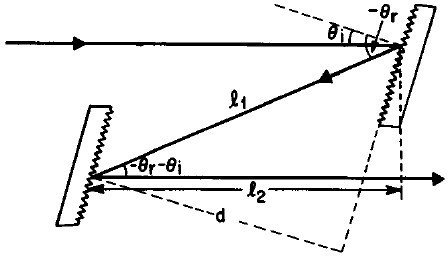
\includegraphics[width=0.5\linewidth]{reflective grating compressor.jpg}
\caption{Reflective grating dechirper/stretcher \cite{Agrawal2008}.}
\label{fig:RGC}
\end{figure}

For the grating, the accumulated phase considers not only the geometric path length but also the grating phase. The first grating does not add any grating phase because all spectral components are diffracted at the same position. However, the second one imposes a grating phase because different spectral components are now diffracted at different positions of the grating. To calculate the grating phase, only the relative position matters.

\begin{figure}[htbp]
\centering
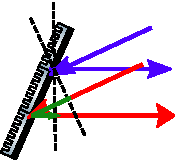
\includegraphics[width=0.2\linewidth]{reflective Treacy_grating phase.pdf}
\caption{The grating phase of a Treacy-type reflective grating dechirper/stretcher.}
\label{fig:reflective_Treacy_grating_phase}
\end{figure}

Because of diffraction after the first grating, the red light propagates farther than the blue light (Fig.~\ref{fig:reflective_Treacy_grating_phase}). This extra propagation phase (from the green line in Fig.~\ref{fig:reflective_Treacy_grating_phase}) needs to be canceled so that it is directed horizontally after the grating. As a result, the grating phase follows
\begin{equation}
\phi_g(x)=\pi+m\frac{x}{\Lambda}2\pi.
\end{equation}
$\pi$ is due to the reflection and will be taken out if we use transmissive gratings. $x$ is the relative position on the grating plane, which in the case of a reflective grating dechirper/stretcher, becomes $d\tan(-\theta_{\text{out}})$. Therefore, the single-pass phase $\phi_{\text{single-pass}}$ becomes
\begin{align}
\phi_{\text{single-pass}} & =k\ell+\phi_g \nonumber \\
& =k\ell+\left[\pi+m\frac{2\pi d\tan(-\theta_{\text{out}})}{\Lambda}\right] \nonumber \\
& =kd\left(\sec\theta_{\text{out}}+\cos\theta_{\text{in}}-\sin\theta_{\text{in}}\tan\theta_{\text{out}}\right)+\left(\pi-m\frac{2\pi d\tan\theta_{\text{out}}}{\Lambda}\right) \nonumber \\
& =kd\left(\sec\theta_{\text{out}}+\cos\theta_{\text{in}}\right)+\pi-d\tan\theta_{\text{out}}\left(k\sin\theta_{\text{in}}+m\frac{2\pi}{\Lambda}\right) \nonumber \\
& =kd\left(\sec\theta_{\text{out}}+\cos\theta_{\text{in}}\right)+\pi-kd\tan\theta_{\text{out}}\sin\theta_{\text{out}} \nonumber \\
& =kd\left(\cos\theta_{\text{out}}+\cos\theta_{\text{in}}\right)+\pi.
\end{align}

To avoid spatial chirp, a mirror is introduced after the first pass of the grating pair so that all spectral components propagate back to where they are, eliminating the spatial chirp. Due to this extra reflecting propagation, the total phase is two times larger, that is,
\begin{equation}
\phi_{\text{double-pass}}=2\left[kd\left(\cos\theta_{\text{out}}+\cos\theta_{\text{in}}\right)+\pi\right].
\end{equation}

\subsection{Transmissive Treacy type}
The derivation follows the reflective grating dechirper/stretcher discussed previously. The total optical path length (Fig.~\ref{fig:TGC}) is
\begin{equation}
\ell=\ell_1+\ell_2=\ell_1+\left[M-\left(M-\ell_2\right)\right].
\end{equation}

\begin{figure}[htbp]
\centering
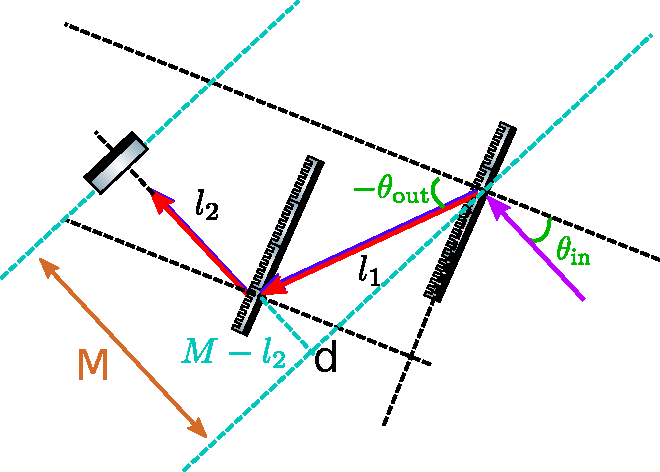
\includegraphics[width=0.5\linewidth]{transmission grating.pdf}
\caption{Transmissive grating dechirper/stretcher.}
\label{fig:TGC}
\end{figure}


Since $M$ is independent of frequency, I keep only the parameters relevant in pulse dechirping/stretching. Hence, $\ell$ becomes
\begin{align}
\ell & =\ell_1+\left[M-\left(M-\ell_2\right)\right] \nonumber \\
& \rightarrow \ell_1-\left(M-\ell_2\right) \nonumber \\
& =\ell_1-\ell_1\sin\left(\frac{\pi}{2}-\theta_{\text{in}}+\theta_{\text{out}}\right) \nonumber \\
& =\ell_1-\ell_1\cos\left(\theta_{\text{in}}-\theta_{\text{out}}\right) \nonumber \\
& =d\sec\theta_{\text{out}}\left[1-\cos(\theta_{\text{in}}-\theta_{\text{out}})\right] \nonumber \\
& =d\sec\theta_{\text{out}}\left(1-\cos\theta_{\text{in}}\cos\theta_{\text{out}}-\sin\theta_{\text{in}}\sin\theta_{\text{out}}\right) \nonumber \\
& =d\left(\sec\theta_{\text{out}}-\cos\theta_{\text{in}}-\sin\theta_{\text{in}}\tan\theta_{\text{out}}\right).
\end{align}

Similar to the reflective gratings, the grating phase from the transmissive grating is added to calculate the single-pass total phase.
\begin{align}
\phi_{\text{single-pass}} & =k\ell+\phi_g=k\ell+m\frac{2\pi d\tan(-\theta_{\text{out}})}{\Lambda} \nonumber \\
& =kd\left(\cos\theta_{\text{out}}-\cos\theta_{\text{in}}\right).
\end{align}

To eliminate the spatial chirp, the total phase after introducing a mirror becomes
\begin{equation}
\phi_{\text{double-pass}}=2\left[kd\left(\cos\theta_{\text{out}}-\cos\theta_{\text{in}}\right)\right].
\end{equation}

\subsection{Group delay dispersion of Treacy dechirper/stretcher}
Here, group delay dispersion (GDD) of both reflective and transmissive grating dechirpers/stretchers are shown. They are used to calculate an initial guess of the grating separation, $d$, for the subsequent grating-pair optimization schemes.
\begin{subequations}
\begin{align}
\dod[2]{\phi_{\text{double-pass}}}{\omega} & =-\frac{m^2\lambda^3d}{\pi c^2\Lambda^2\cos^3\theta_{\text{out}}} \\
\dod[3]{\phi_{\text{double-pass}}}{\omega} & =\frac{3m^2\lambda^4d\left(1+\sin\theta_{\text{in}}\sin\theta_{\text{out}}\right)}{2\pi^2c^3\Lambda^2\cos^5\theta_{\text{out}}}
\end{align}
\end{subequations}
where $m$ is the diffraction order and is typically $-1$, $\lambda$ is the pulse center wavelength, $d$ is the grating separation, and $\Lambda$ is the grating line spacing.

\section{Prism type}
As grating pair, prism pair that disperses color can be used as a dechirper or stretcher. It operates as in Fig.~\ref{fig:prism}. The light should hit the prism as close to the apex as possible.
\begin{figure}[htbp]
\centering
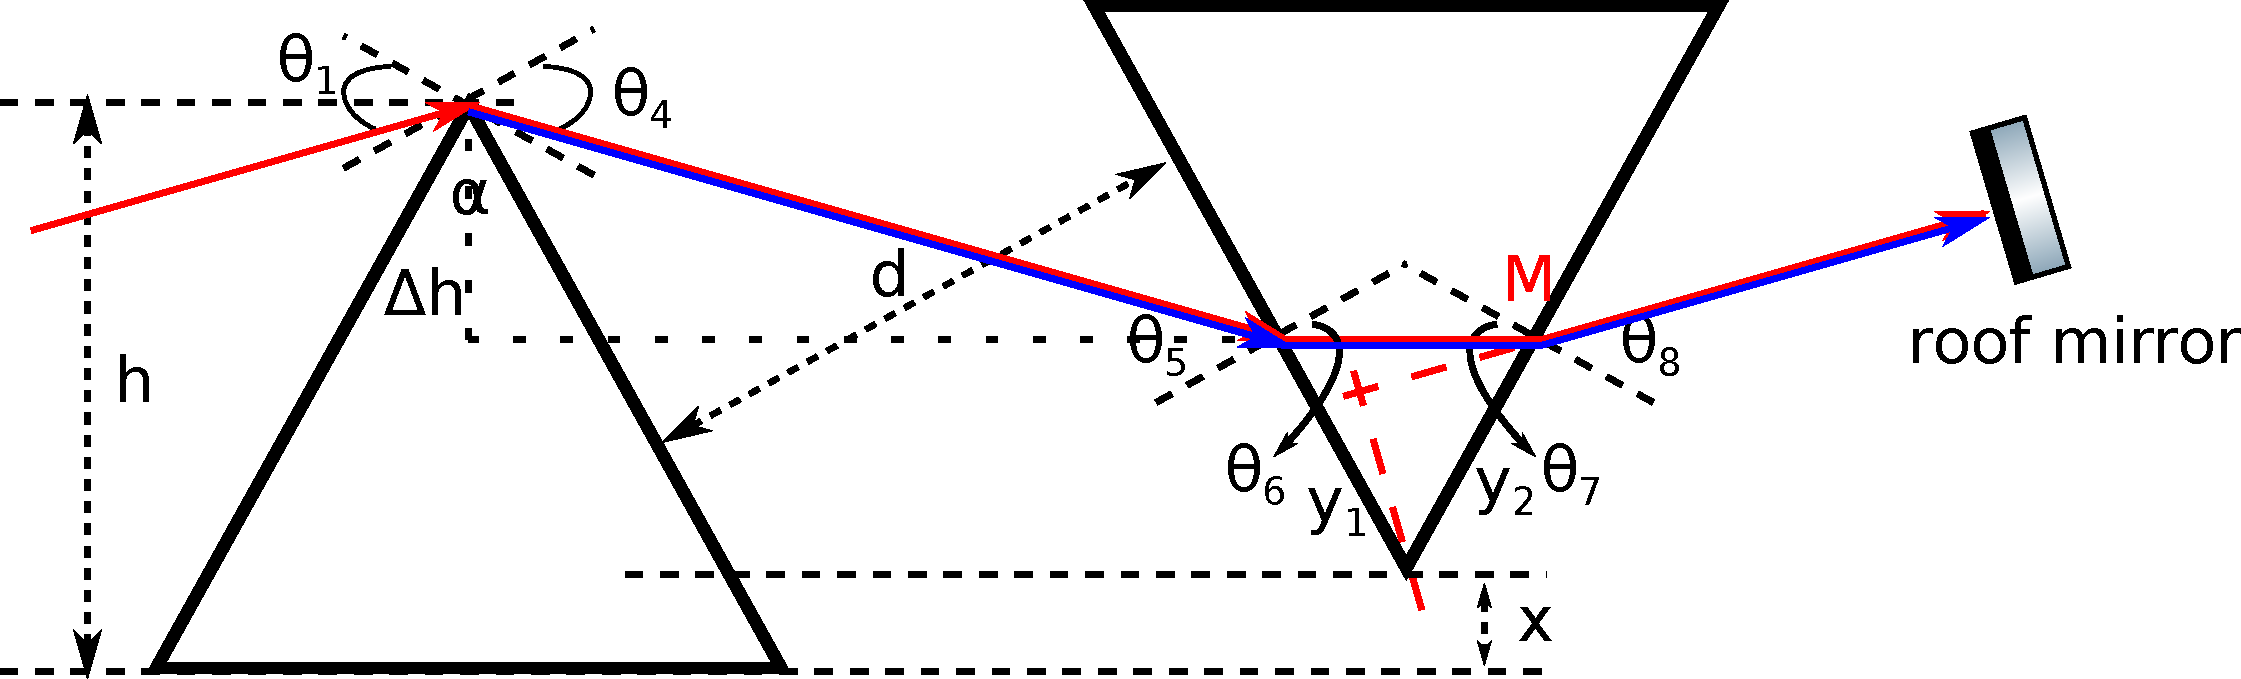
\includegraphics[width=\linewidth]{prism.pdf}
\caption{Prism dechirper/stretcher.}
\label{fig:prism}
\end{figure}

In principle, the $\alpha$ angle can be varied to tune the dispersion properties of a prism dechirper/stretcher. In practice, however, the geometry is chosen such that the incident and refracted beam have the same angle at the central wavelength of the spectrum to be dechirped/stretched. This configuration is known as the ``angle of minimum deviation,'' and is easier to align than arbitrary angles (Fig.~\ref{fig:prism_enlarged}). In this configuration, the angles of refraction through the prism are symmetric, that is in Fig.~\ref{fig:prism_enlarged},
\begin{subequations}
\begin{align}
\theta_1=\theta_4 \\
\theta_2=\theta_3=\frac{\alpha}{2}.
\end{align}
\end{subequations}
\begin{figure}[htbp]
\centering
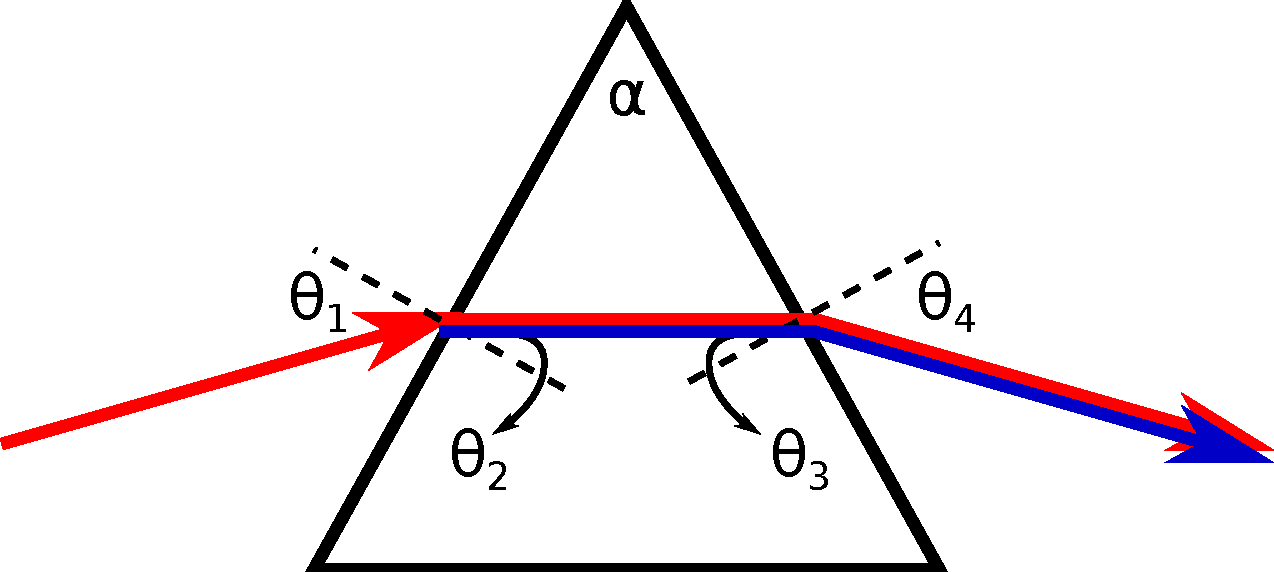
\includegraphics[width=0.4\linewidth]{prism_enlarged.pdf}
\caption{Prism operation with a minimum beam deviation.}
\label{fig:prism_enlarged}
\end{figure}

To calculate the phase added to the pulse, the incident angle needs to be determined so that the beam of its center wavelength $\lambda_0$ enters the configuration of ``angle of minimum deviation:''
\begin{align}
& \sin\theta_{\text{in}}=n(\lambda_0)\sin\theta_2,\quad\text{with }\theta_2=\frac{\alpha}{2} \nonumber \\
&\Rightarrow \theta_{\text{in}}=\sin^{-1}\left(n(\lambda_0)\sin\frac{\alpha}{2}\right). \label{eq:prism_theta_in}
\end{align}

Next, we calculate each angle in Fig.~\ref{fig:prism_enlarged}:
\begin{subequations}
\begin{align}
& n(\lambda)\sin\theta_2=\sin\theta_{\text{in}} \\
&\Rightarrow \theta_3=\alpha-\theta_2 \\
&\Rightarrow \sin\theta_4=n(\lambda)\sin\theta_3.
\end{align}
\end{subequations}
With calculated $\theta_4$ for each wavelength, we subsequently obtain
\begin{subequations}
\begin{align}
& \theta_5=\theta_4 \\
&\Rightarrow n(\lambda)\sin\theta_6=\sin\theta_5 \\
&\Rightarrow \theta_7=\alpha-\theta_6 \\
&\Rightarrow \sin\theta_8=n(\lambda)\sin\theta_7.
\end{align}
\end{subequations}
These lead to
\begin{subequations}
\begin{align}
\theta_5 & =\theta_4 \\
\theta_6 & =\theta_3 \\
\theta_7 & =\theta_2 \\
\theta_8 & =\theta_1=\theta_{\text{in}}. \label{eq:prism_theta8}
\end{align}
\label{eq:prism_theta_equivalent}
\end{subequations}
Eq.~(\ref{eq:prism_theta8}) shows that all the colors exit the second prism with the same angle such that they can all be reflected back to their original paths after the roof mirror. 

To find the path lengths after entering the second prism, we need to calculate the change of height of the beam when hitting the second prism. It is $\triangle h=\ell_s\cos(\frac{\pi}{2}-\theta_4+\frac{\alpha}{2})=\ell_s\sin(\theta_4-\frac{\alpha}{2})$, where the path length between two prisms is $\ell_s=d\sec(\theta_4)$, leading to $\triangle h=d\left(\tan\theta_4\cos\frac{\alpha}{2}-\sin\frac{\alpha}{2}\right)$. The distance between where the beam hitting the prism and the apex of the second prism is $y_1=\left(h-\triangle h-x\right)\sec\frac{\alpha}{2}$. It allows us to find the path length to travel inside the second prism $\ell_p$ and the length on the hypotenuse $y_2$ through the following relation:
\begin{equation}
\frac{y_1}{\sin(\frac{\pi}{2}-\theta_7)}=\frac{\ell_p}{\sin\alpha}=\frac{y_2}{\sin(\frac{\pi}{2}-\theta_6)}.
\end{equation}
And thus
\begin{subequations}
\begin{align}
\ell_p & =\frac{y_1\sin\alpha}{\cos\theta_2} \\
y_2 & =\frac{y_1\cos\theta_3}{\cos\theta_2}
\end{align}
\label{eq:prism_lpy2}
\end{subequations}
$y_2$ contributes to the change of path length to the roof mirror by $\ell_M=M-y_2\cos(\frac{\pi}{2}-\theta_8)=M-y_2\sin\theta_{\text{in}}\sim-y_2\sin\theta_{\text{in}}$.

In conclusion, the path lengths to consider are
\begin{subequations}
\begin{align}
\ell_s & =d\sec\theta_4 \\
\ell_p & =\frac{y_1\sin\alpha}{\cos\theta_2}=\frac{\left(h-\triangle h-x\right)\sec\frac{\alpha}{2}\sin\alpha}{\cos\theta_2}=\frac{2\left(h-\triangle h-x\right)\sin\frac{\alpha}{2}}{\cos\theta_2} \\
\ell_M & =-y_2\sin\theta_{\text{in}}=-\frac{y_1\cos\theta_3}{\cos\theta_2}\sin\theta_{\text{in}}=-\frac{\left(h-\triangle h-x\right)\cos\theta_3}{\cos\frac{\alpha}{2}\cos\theta_2}\sin\theta_{\text{in}} \\
& =-\frac{\left(h-\triangle h-x\right)\left(\cos\alpha+\sin\alpha\tan\theta_2\right)}{\cos\frac{\alpha}{2}}\sin\theta_{\text{in}}
\end{align}
\end{subequations}

As a result, the total phase of this prism dechirper/stretcher is
\begin{equation}
\phi_{\text{double-pass}}=2k\left(\ell_s+n\ell_p+\ell_M\right).
\end{equation}

$x$ is picked so that the dispersed beam hits the apex of the second prism such that $\min_{\lambda\in\text{pulse spectrum}} y_1(\lambda)=0$.

\subsection{Group delay dispersion of prism dechirper/stretcher}
From \cite{Fork1984}, the path length that determines the GDD added to the pulse is 
\begin{equation}
P=2\ell\cos\beta,
\end{equation}
where $\ell$ is the length between apexes of two prisms, and $\beta$ is the angle of the beam with respect to the line connecting two apexes (Fig.~\ref{fig:prism_GDD}). The corresponding GDD is
\begin{align}
\dod[2]{\phi}{\omega} & =\frac{\lambda^3}{2\pi c^2}\dod[2]{P(\lambda)}{\lambda} \nonumber \\
& =\frac{\lambda^3}{2\pi c^2}4\ell\left\{\left[\dod[2]{n}{\lambda}+\left(2n-\frac{1}{n^3}\right)\left(\dod{n}{\lambda}\right)^2\right]\sin\beta-2\left(\dod{n}{\lambda}\right)^2\cos\beta\right\},
\label{eq:prism_GDD}
\end{align}
where $n$ is the refractive index of the prism material.
\begin{figure}[htbp]
\centering
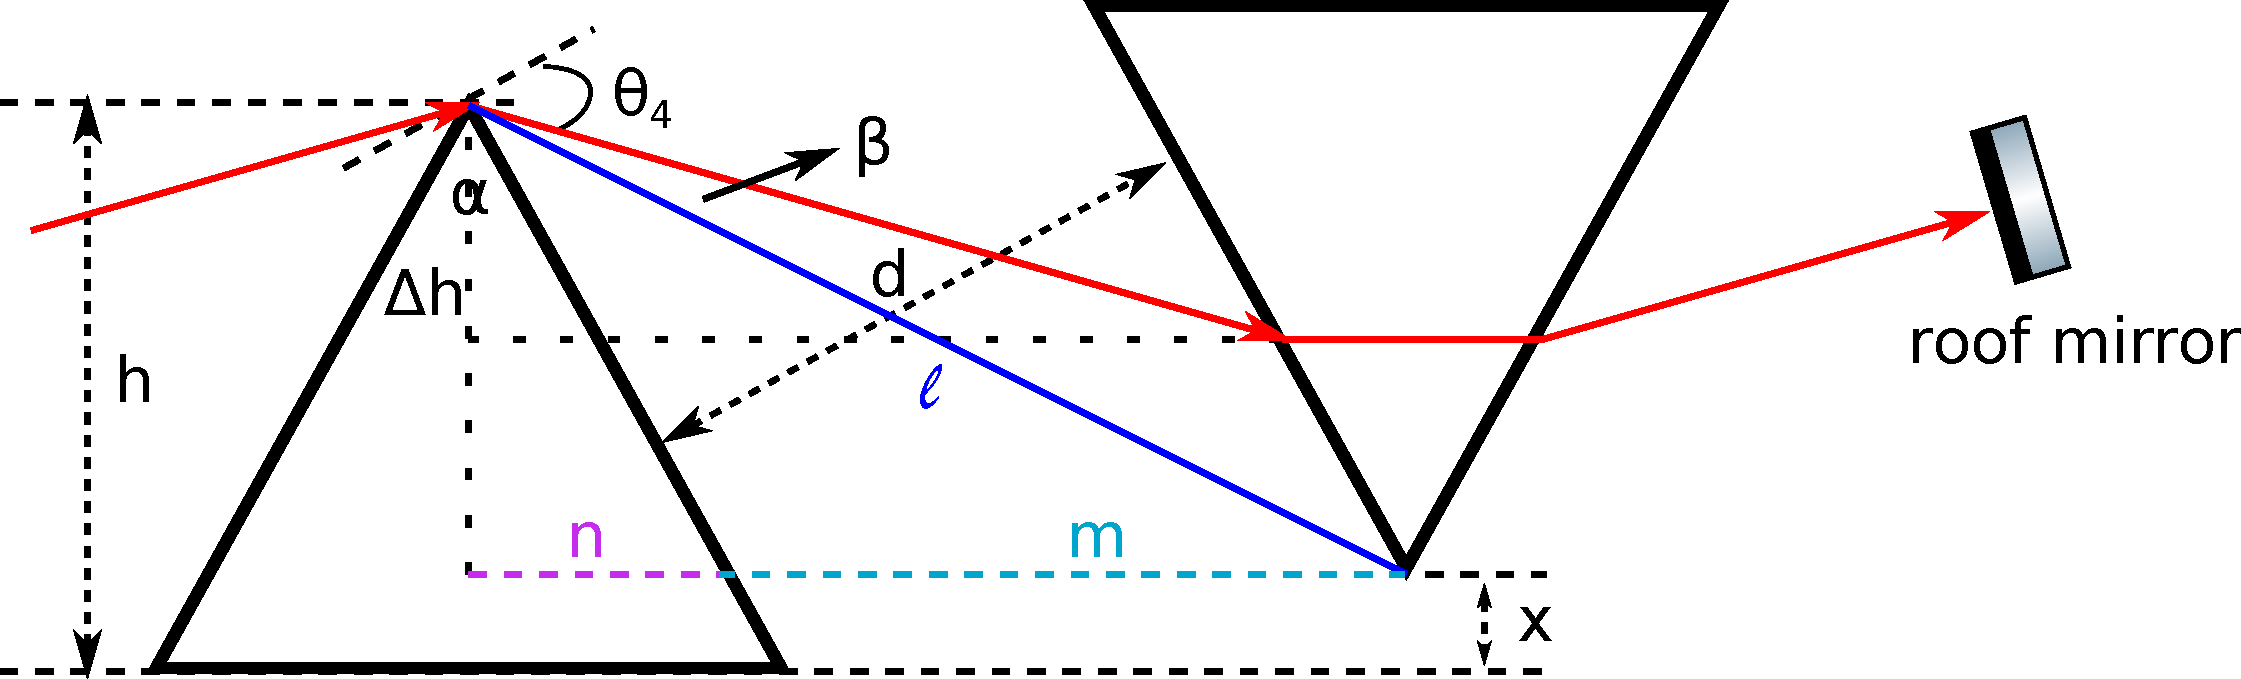
\includegraphics[width=\linewidth]{prism_GDD.pdf}
\caption{Schematic for calculating the prism GDD.}
\label{fig:prism_GDD}
\end{figure}

To find the value of Eq.~(\ref{eq:prism_GDD}), we need to determine $\ell$ and $\beta$ that depend on the prism separation $d$, pulse bluest wavelength $\lambda_b$, and its center wavelength $\lambda_0$. In prism operations, the blue edge of the light is, in principle, put near the apex of the second prism, which leads to
\begin{subequations}
\begin{align}
\ell & =\ell_s(\lambda_b)=d\sec\theta_4(\lambda_b) \\
\beta & =\theta_4(\lambda_b)-\theta_4(\lambda_0).
\end{align}
\end{subequations}

Finally, we obtain
\begin{align}
\dod[2]{\phi}{\omega}(\lambda_0) & =\frac{\lambda_0^3}{2\pi c^2}\dod[2]{P(\lambda_0)}{\lambda} \nonumber \\
&\hspace{-2em} =\frac{\lambda_0^3}{2\pi c^2}4d\sec\theta_4(\lambda_b) \nonumber \\
&\hspace{-1em} \times\left\{\left[\dod[2]{n}{\lambda}(\lambda_0)+\left(2n(\lambda_0)-\frac{1}{\left(n(\lambda_0)\right)^3}\right)\left(\dod{n}{\lambda}(\lambda_0)\right)^2\right]\sin\beta-2\left(\dod{n}{\lambda}(\lambda_0)\right)^2\cos\beta\right\}.
\label{eq:prism_GDD2}
\end{align}

\section{Grism type}
Grating-based stretchers/dechirpers have the opposite sign of GDD and TOD, leading to more TOD after dechirping a fiber-stretched pulse. As a result, it is desirable to have a dechirper that has the same sign of GDD and TOD. Although prism dechirper meets the need, its GDD is too weak for huge dechirping. Therefore, a combination of prism and grating is proposed \cite{Tournois1993,Kane1997,Dou2010,Forget2012}.

\subsection{Configuration 1}
Grism can be operated differently. Here I employ one operation that follows Fig.~\ref{fig:grism}, where a transmission grating is attached before the right-angle prism.

\begin{figure}[htbp]
\centering
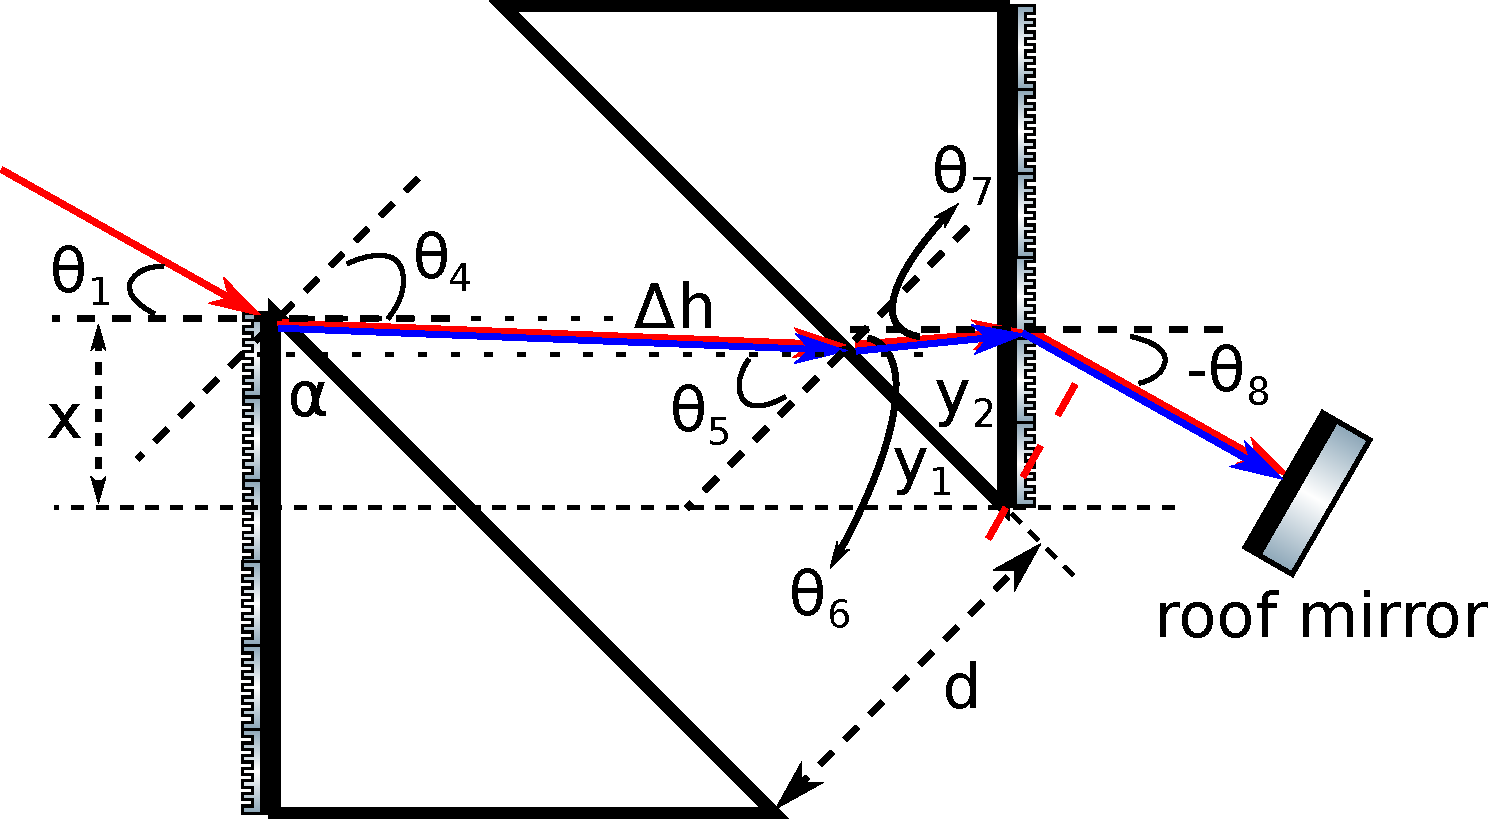
\includegraphics[width=.7\linewidth]{grism v2.pdf}
\caption{Grism dechirper/stretcher.}
\label{fig:grism}
\end{figure}

\begin{figure}[htbp]
\centering
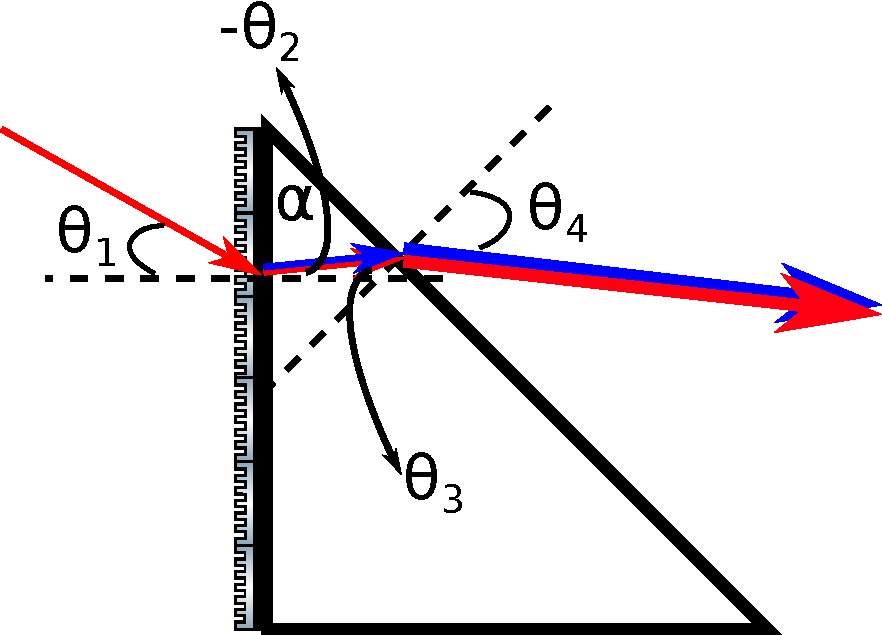
\includegraphics[width=0.4\linewidth]{grism_enlarged v2.pdf}
\caption{One of grism operations with a transmission grating.}
\label{fig:grism_enlarged}
\end{figure}

Similar to prism stretcher/dechirper [Eqs.~(\ref{eq:prism_theta_equivalent})],
\begin{subequations}
\begin{align}
\theta_5 & =\theta_4 \\
\theta_6 & =\theta_3 \\
\theta_7 & =-\theta_2 \\
-\theta_8 & =\theta_1=\theta_{\text{in}}.
\end{align}
\end{subequations}
Also,
\begin{subequations}
\begin{align}
& \Lambda\left(n(\lambda)\sin\theta_2-\sin\theta_{\text{in}}\right)=m\lambda \nonumber \\
&\Rightarrow \sin\theta_2=\frac{1}{n(\lambda)}\left(m\frac{\lambda}{\Lambda}+\sin\theta_{\text{in}}\right) \\[0.5em]
& \theta_3=\alpha+\theta_2 \\
& \sin\theta_4=n(\lambda)\sin\theta_3
\end{align}
\end{subequations}

The path length between two prisms is $\ell_s=d\sec\theta_4$. The vertical translation of the beam is $\triangle h=\ell_s\sin\left(\theta_4-\alpha\right)=d\left(\tan\theta_4\cos\alpha-\sin\alpha\right)$.

To find the path length inside the prism, we need the following relation:
\begin{equation}
\frac{\ell_p}{\sin\alpha}=\frac{y_1}{\sin\left(\frac{\pi}{2}-\theta_7\right)}=\frac{y_2}{\sin\left(\frac{\pi}{2}-\theta_6\right)}.
\end{equation}
With $y_1=\left(x-\triangle h\right)\sec\alpha$, we obtain 
\begin{subequations}
\begin{align}
\ell_p & =\frac{y_1\sin\alpha}{\cos\theta_7}=\frac{x-\triangle h}{\cos\theta_7}\tan\alpha \\
y_2 & =\frac{y_1\cos\theta_6}{\cos\theta_7}=\frac{\left(x-\triangle h\right)\cos\theta_6}{\cos\theta_7}\sec\alpha.
\end{align}
\end{subequations}

In addition, the grating phase $\displaystyle \phi_g=m\frac{y_2}{\Lambda}2\pi$ needs to be considered.

In conclusion, the path lengths to consider are
\begin{subequations}
\begin{align}
\ell_s & =d\sec\theta_4 \\
\ell_p & =\frac{y_1\sin\alpha}{\cos\theta_7}=\frac{x-\triangle h}{\cos\theta_2}\tan\alpha \\
\ell_M & =y_2\cos(\frac{\pi}{2}+\theta_8)=\frac{\left(x-\triangle h\right)\cos\theta_3}{\cos\theta_2}\sec\alpha\sin\theta_{\text{in}} \nonumber \\
& =\left(x-\triangle h\right)\left(\cos\alpha-\sin\alpha\tan\theta_2\right)\sec\alpha\sin\theta_{\text{in}}
\end{align}
\end{subequations}

As a result, the total phase of this prism dechirper/stretcher is
\begin{equation}
\phi_{\text{double-pass}}=2\left[k\left(\ell_s+n\ell_p+\ell_M\right)+\phi_g\right].
\end{equation}

Similar to the prism dechirper/stretcher, $x$ is picked so that the dispersed beam hits the apex of the second prism such that $\min_{\lambda\in\text{pulse spectrum}} y_1(\lambda)=0$.

\subsection{Configuration 2}
In this section, I employ another operation that follows Fig.~\ref{fig:grism2}. In contrast to Fig.~\ref{fig:grism}, prisms are operated with minimum deviation for the pulse center wavelength as a prism dechirper/stretcher. Therefore, gratings cannot be attached to prisms.

\begin{figure}[htbp]
\centering
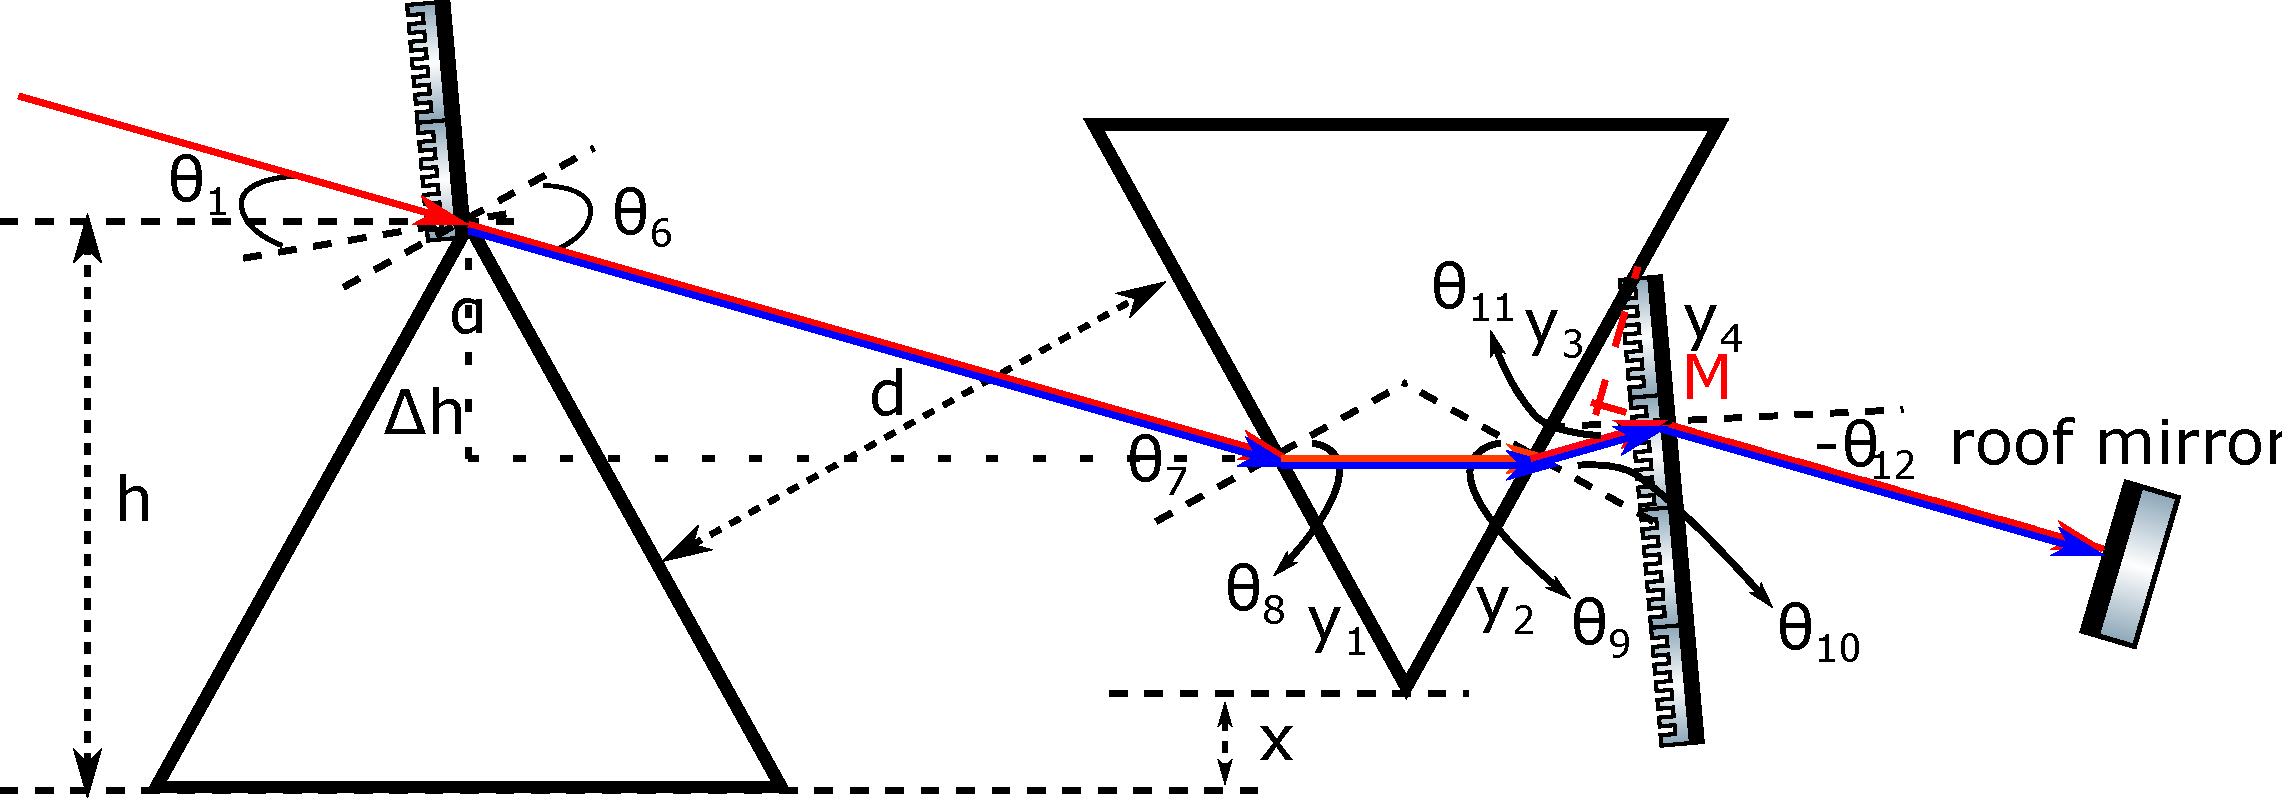
\includegraphics[width=.7\linewidth]{grism v3.pdf}
\caption{Grism dechirper/stretcher.}
\label{fig:grism2}
\end{figure}

\begin{figure}[htbp]
\centering
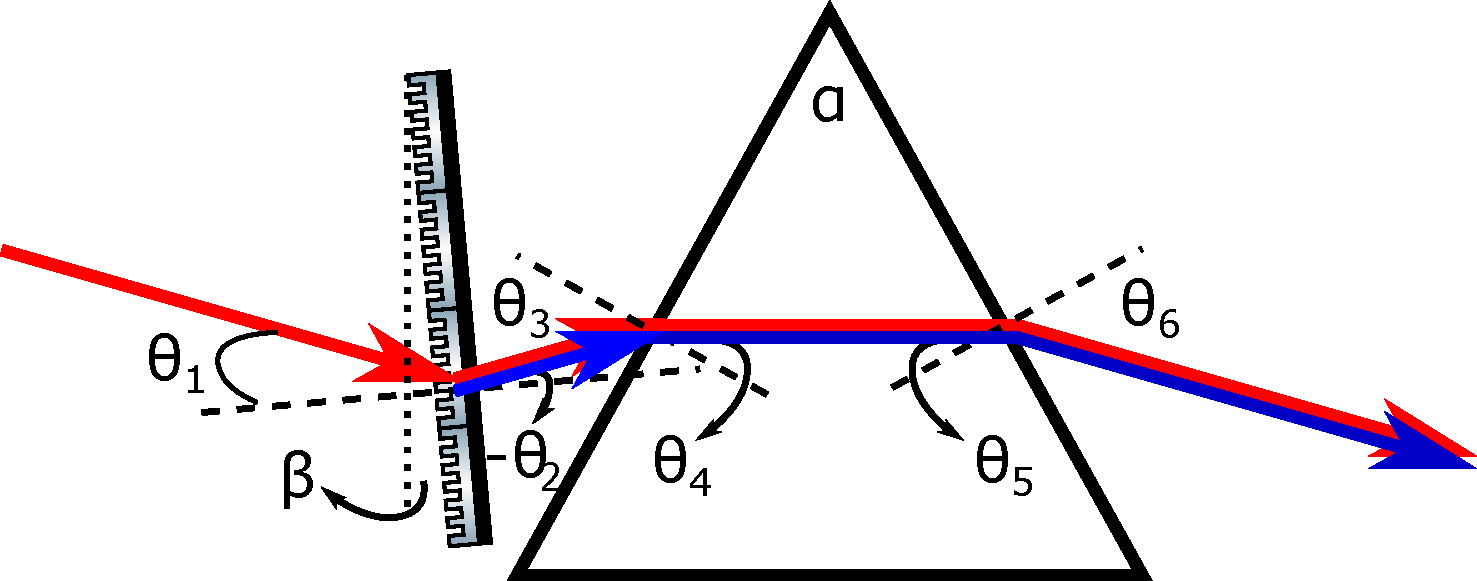
\includegraphics[width=0.4\linewidth]{grism_enlarged v3.pdf}
\caption{One of grism operations with a transmission grating.}
\label{fig:grism_enlarged2}
\end{figure}

Similar to prism stretcher/dechirper [Eqs.~(\ref{eq:prism_theta_equivalent})],
\begingroup\allowdisplaybreaks
\begin{subequations}
\begin{align}
\theta_7 & =\theta_6 \\
\theta_8 & =\theta_5 \\
\theta_9 & =\theta_4 \\
\theta_{10} & =\theta_3 \\
\theta_{11} & =-\theta_2 \\
-\theta_{12} & =\theta_1=\theta_{\text{in}}.
\end{align}
\end{subequations}
\endgroup
Also,
\begin{subequations}
\begin{align}
& \Lambda\left(\sin\theta_2-\sin\theta_{\text{in}}\right)=m\lambda \nonumber \\
&\Rightarrow \sin\theta_2=m\frac{\lambda}{\Lambda}+\sin\theta_{\text{in}} \\[0.5em]
& \theta_3=\frac{\alpha}{2}+\beta-\theta_2 \label{eq:theta3_grism2} \\
& n(\lambda)\sin\theta_4=\sin\theta_3 \\
& \theta_5=\alpha-\theta_4 \\
& \sin\theta_6=n(\lambda)\sin\theta_5
\end{align}
\end{subequations}

The path length between two prisms is $\ell_s=d\sec\theta_6$. The vertical translation of the beam is $\triangle h=\ell_s\cos(\frac{\pi}{2}-\theta_6+\frac{\alpha}{2})=\ell_s\sin(\theta_6-\frac{\alpha}{2})=d\left(\tan\theta_6\cos\frac{\alpha}{2}-\sin\frac{\alpha}{2}\right)$.

To find the path length inside the prism, we need the following relation:
\begin{equation}
\frac{\ell_p}{\sin\alpha}=\frac{y_1}{\sin\left(\frac{\pi}{2}-\theta_9\right)}=\frac{y_2}{\sin\left(\frac{\pi}{2}-\theta_8\right)}.
\end{equation}
With $y_1=\left(h-x-\triangle h\right)\sec\frac{\alpha}{2}$, we obtain 
\begin{subequations}
\begin{align}
\ell_p & =\frac{y_1\sin\alpha}{\cos\theta_9}=\frac{h-x-\triangle h}{\cos\theta_9}\sin\alpha\sec\frac{\alpha}{2}=2\frac{h-x-\triangle h}{\cos\theta_9}\sin\frac{\alpha}{2} \\
y_2 & =\frac{y_1\cos\theta_8}{\cos\theta_9}=\frac{\left(h-x-\triangle h\right)\cos\theta_8}{\cos\theta_9}\sec\frac{\alpha}{2}.
\end{align}
\end{subequations}

To find the path length between the prism and the grating, we use:
\begin{equation}
\frac{\ell_{pg}}{\sin(\frac{\alpha}{2}+\beta)}=\frac{y_3-y_2}{\sin(\frac{\pi}{2}+\theta_{11})}=\frac{y_4}{\sin(\frac{\pi}{2}-\theta_{10})},
\end{equation}
which gives us
\begin{subequations}
\begin{align}
\ell_{pg} & =\frac{y_3-y_2}{\sin(\frac{\pi}{2}+\theta_{11})}\sin(\frac{\alpha}{2}+\beta)=\frac{y_3-y_2}{\cos\theta_{11}}\sin(\frac{\alpha}{2}+\beta) \\
y_4 & =\frac{y_3-y_2}{\sin(\frac{\pi}{2}+\theta_{11})}\sin(\frac{\pi}{2}-\theta_{10})=\frac{y_3-y_2}{\cos\theta_{11}}\cos\theta_{10}
\end{align}
\end{subequations}

In addition, the grating phase $\displaystyle \phi_g=m\frac{-y_4}{\Lambda}2\pi$ needs to be considered.

In conclusion, the path lengths to consider are
\begin{subequations}
\begin{align}
\ell_s & =d\sec\theta_6 \\
\ell_p & =\frac{y_1\sin\alpha}{\cos\theta_4} \\
\ell_{pg} & =\frac{y_3-y_2}{\cos\theta_2}\sin(\frac{\alpha}{2}+\beta) \\
\ell_M & =-y_4\cos(\frac{\pi}{2}+\theta_{12})=-y_4\sin\theta_{\text{in}}
\end{align}
\end{subequations}

As a result, the total phase of this prism dechirper/stretcher is
\begin{equation}
\phi_{\text{double-pass}}=2\left[k\left(\ell_s+n\ell_p+\ell_{pg}+\ell_M\right)+\phi_g\right].
\end{equation}

Similar to the prism dechirper/stretcher or the previous configuration 1 of grism, $x$ is picked so that the dispersed beam hits the apex of the second prism such that $\min_{\lambda\in\text{pulse spectrum}} y_1(\lambda)=0$. Besides, the second grating is placed to minimize $\ell_{pg}$ which is dominated by grating dechirper/stretcher introducing unwanted positive TOD, so $\min_{\lambda\in\text{pulse spectrum}}\left[y_3(\lambda)-y_2(\lambda)\right]=0$.

Due to the requirement of minimum deviation, $\theta_4(\lambda_0)=\frac{\alpha}{2}$, leading to $\theta_3(\lambda_0)=\sin^{-1}(n(\lambda_0)\sin\frac{\alpha}{2})$. Because $\sin\theta_2(\lambda_0)=m\frac{\lambda}{\Lambda}+\sin\theta_{\text{in}}$ and Eq.~(\ref{eq:theta3_grism2}), the tilt angle of gratins $\beta$ can be determined so that the diffracted beam satisfies the operation of minimum deviation for prisms.

\section{Martinez type}
Unlike the Treacy and prism types that add only negative chirp, Martinez type can add an arbitrary sign of chirp based on the relationship between the focal length $f$, and the distance $\ell$, between the grating and the lens (Fig.~\ref{fig:martinez_stretcher}). It adds positive chirp (corresponding to normal dispersion) when $\ell<f$ and negative chirp (corresponding to anomalous dispersion) when $\ell>f$; nothing happens when $\ell=f$ which is simply a 4f-telescope. It is often used as a pulse stretcher for chirped pulse amplification while a Treacy type is for latter pulse dechirper to cancel the chirp added by the Martinez stretcher.

\begin{figure}[htbp]
\centering
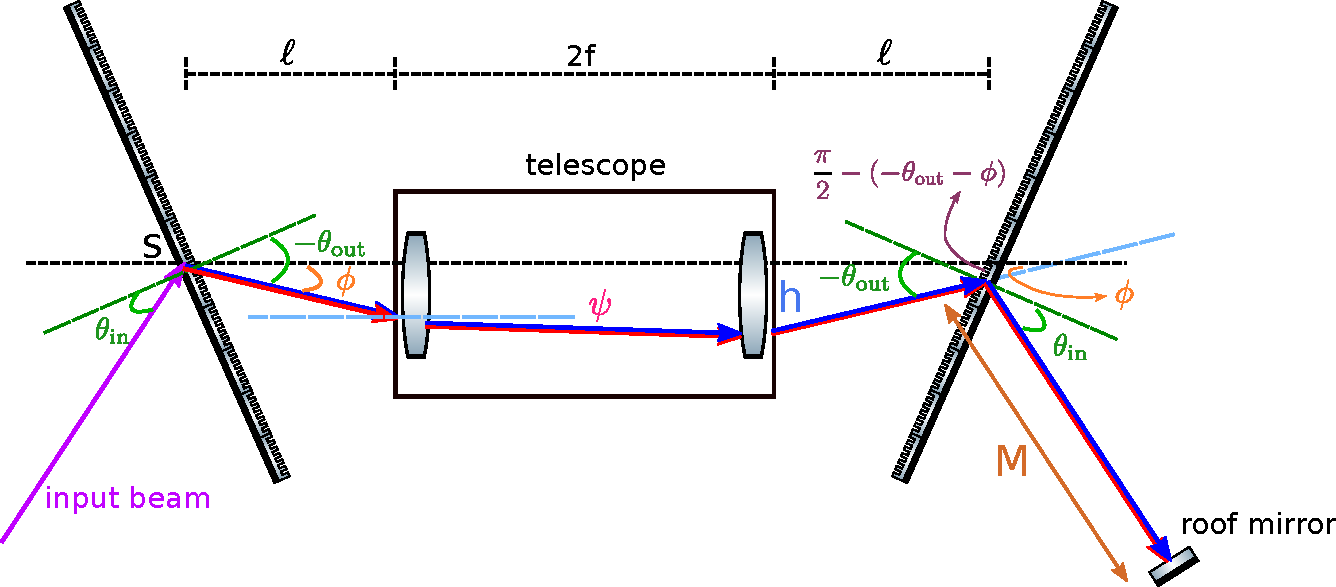
\includegraphics[width=\textwidth]{Martinez stretcher.pdf}
\caption{Martinez dechirper/stretcher.}
\label{fig:martinez_stretcher}
\end{figure}

There are four path lengths required in the phase calculation: $\ell_1$, the first grating to the first lens; $\ell_2$, the distance between two lenses; $\ell_3$, the second lens to the second grating; $\ell_4$, the second grating to the roof mirror for a second pass of the entire system to cancel the introduced spatial chirp after a single pass.

To calculate the first path length $\ell_1=\ell\sec\phi$, we need to calculate the relative diffraction angle $\phi$. Because the alignment of the telescope is determined by the center wavelength of the input signal, we need to first determine the ``center'' diffraction angle to calculate $\phi$. From here, we can see that the actual value of $\phi$ can be quite arbitrary. 

To calculate the second path length $\ell_2=2f\sec\psi$, we calculate $\psi$ with ABCD matrices.
\begin{subequations}
\begin{align}
& T_{\text{lens}}=\begin{bmatrix}
1 & 0 \\
-\frac{1}{f} & 1
\end{bmatrix}
\begin{bmatrix}
1 & \ell \\
0 & 1
\end{bmatrix}=
\begin{bmatrix}
1 & \ell \\
-\frac{1}{f} & -\frac{\ell}{f}+1
\end{bmatrix} \\
& T_{\text{lens}}
\begin{bmatrix}
0 \\ \phi
\end{bmatrix}=
\begin{bmatrix}
\ell\phi \\ \left(1-\frac{\ell}{f}\right)\phi
\end{bmatrix}=
\begin{bmatrix}
\ell\tan\phi \\ \left[1-\tan^{-1}\left(\frac{\ell}{f}\right)\right]\phi
\end{bmatrix},
\end{align}
\end{subequations}
which leads to
\begin{equation}
\psi=\left(1-\frac{\ell}{f}\right)\phi=\left[1-\tan^{-1}\left(\frac{\ell}{f}\right)\right]\phi\text{, }\tan^{-1}\text{ is more accurate}
\end{equation}

Before we calculate the third path length $\ell_3$, we are interested in the light passing through the telescope.
\begin{subequations}
\begin{align}
& T=\begin{bmatrix}
1 & 0 \\
-\frac{1}{f} & 1
\end{bmatrix}
\begin{bmatrix}
1 & 2f \\
0 & 1
\end{bmatrix}
\begin{bmatrix}
1 & 0 \\
-\frac{1}{f} & 1
\end{bmatrix}
\begin{bmatrix}
1 & \ell \\
0 & 1
\end{bmatrix}=
\begin{bmatrix}
-1 & 2f-\ell \\
0 & -1
\end{bmatrix} \\
& \Rightarrow\quad T
\begin{bmatrix}
0 \\ \phi
\end{bmatrix}=
\begin{bmatrix}
(2f-\ell)\phi \\ -\phi
\end{bmatrix}
\end{align}
\end{subequations}
This shows that the light maintains the same output angle as the input angle but with a vertical offset $h=(2f-\ell)\phi=(2f-\ell)\tan\phi$.

To calculate the third path length $\ell_3=h\csc\phi-x$, we need to calculate $x$ (Fig.~\ref{fig:martinez_stretcher_close_view}).
\begin{figure}[htbp]
\centering
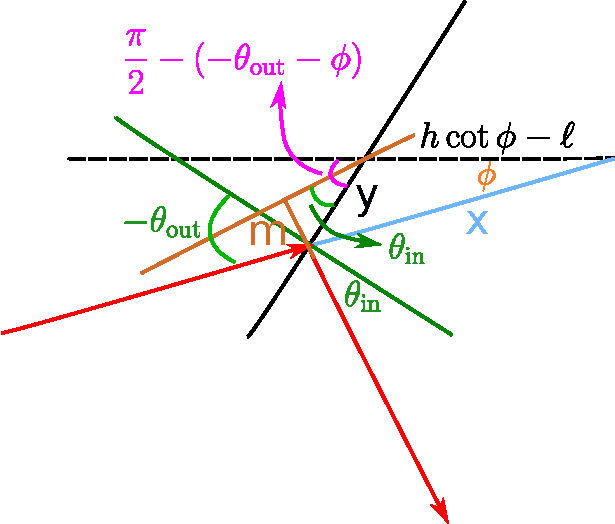
\includegraphics[width=.4\textwidth]{Martinez stretcher (close view).pdf}
\caption{Diagram of a Martinez dechirper/stretcher to calculate the propagation length.}
\label{fig:martinez_stretcher_close_view}
\end{figure}
\begin{align}
& \frac{h\cot\phi-\ell}{\sin\left(\frac{\pi}{2}-\left(-\theta_{\text{out}}-\phi\right)-\phi\right)}=\frac{x}{\sin\left(\frac{\pi}{2}-\left(-\theta_{\text{out}}-\phi\right)\right)}=\frac{y}{\sin\phi} \nonumber \\
& \Rightarrow\quad\frac{h\cot\phi-\ell}{\cos\theta_{\text{out}}}=\frac{x}{\cos\left(\theta_{\text{out}}+\phi\right)}=\frac{y}{\sin\phi} \label{eq:martinez_xy}
\end{align}
However, $h\cot\phi$ term can create NaN (``not a number'' in MATLAB) during computation. When $\phi=0$, $h=0$; this term becomes $0\times\infty$. To avoid the ambiguity, it is preferable to use $h\cot\phi=2f-\ell$. Thus, the relation above becomes
\begin{equation}
\frac{2(f-\ell)}{\cos\theta_{\text{out}}}=\frac{x}{\cos\left(\theta_{\text{out}}+\phi\right)}=\frac{y}{\sin\phi},
\end{equation}
which gives
\begin{subequations}
\begin{align}
x & =\frac{2(f-\ell)}{\cos\theta_{\text{out}}}\cos\left(\theta_{\text{out}}+\phi\right) \\
y & =\frac{2(f-\ell)}{\cos\theta_{\text{out}}}\sin\phi.
\end{align}
\end{subequations}

The last path length is $\ell_4=M-m$, where $m=y\sin\theta_{\text{in}}$.

Therefore, the single-pass path length is 
\begin{align}
\ell_{\text{single-pass}} & =\ell\sec\phi+2f\sec\psi+h\csc\phi-x+M-y\sin\theta_{\text{in}} \nonumber \\
& \rightarrow \ell\sec\phi+2f\sec\psi+h\csc\phi-x-y\sin\theta_{\text{in}}.
\end{align}

Similarly, there is a grating phase (Fig.~\ref{fig:transmissive_Martinez_grating_phase})
\begin{equation}
\phi_g=-m\frac{y}{\Lambda}2\pi.
\end{equation}
\begin{figure}[htbp]
\centering
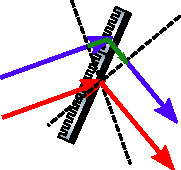
\includegraphics[scale=1]{transmissive Martinez_grating phase.pdf}
\caption{The grating phase of an Martinez-type transmissive grating dechirper/stertcher.}
\label{fig:transmissive_Martinez_grating_phase}
\end{figure}

Besides the above obvious optical path length and grating phase, there is another phase required to be taken into account: the lens phase, or the lens-thickness optical path length. This explains why the light direction changes after it passes through a lens with Huygens principle. It adds a phase to the light incident on different positions of a lens and thus bends the light, similar to a grating. Since the light from the focus travels in collimation (having a flat phase front) after a lens, the lens path length can be calculated as
\begin{subequations}
\begin{align}
& \text{The \nth{1} lens: }\ell_{\text{lens 1}}=-\sqrt{h_{\text{lens 1}}^2+f^2}=-\sqrt{(\ell\tan\phi)^2+f^2} \\
& \text{The \nth{2} lens: }\ell_{\text{lens 2}}=-\sqrt{h_{\text{lens 2}}^2+f^2}=-\sqrt{h^2+f^2}.
\end{align}
\end{subequations}
\begin{equation}
\ell_{\text{lens}}=\ell_{\text{lens 1}}+\ell_{\text{lens 2}}=-\sqrt{(\ell\tan\phi)^2+f^2}-\sqrt{h^2+f^2}.
\end{equation}
Thus, the single-pass total phase is
\begin{equation}
\phi_{\text{single-pass}}=k\ell_{\text{single-pass}}+k\ell_{\text{lens}}+\phi_g.
\end{equation}
To eliminate spatial chirp, two passes are required. Finally, the double-pass total phase is
\begin{equation}
\phi_{\text{double-pass}}=2\left(k\ell_{\text{single-pass}}+k\ell_{\text{lens}}+\phi_g\right).
\end{equation}

\section{Offner type}
A typical Martinez stretcher relies on a telescope (Fig. \ref{fig:martinez_stretcher}) but these refractive components can introduce aberration for broadband pulses \cite{Cheriaux1996}; therefore, Offner stretcher is preferred due to the use of all reflective optical components (Fig. \ref{fig:Offner_stretcher}).

\begin{figure}[htbp]
\centering
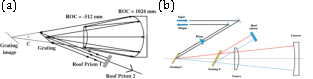
\includegraphics[width=\textwidth]{Offner stretcher.pdf}
\caption{(a) Single-grating \cite{Cheriaux1996} and (b) double-grating reflective Offner dechirpers/stretchers \cite{Liu2020}.}
\label{fig:Offner_stretcher}
\end{figure}

\subsection{Transmissive single-grating Offner type}
I first calculate the accumulated phase of an Offner stretcher with a single transmissive grating (Fig.~\ref{fig:single_Offner_diagram}). There are two concentric convex and concave mirrors, and the transmissive grating is slightly deviated from the center of circles, which introduces abberation.

\begin{figure}[htbp]
\centering
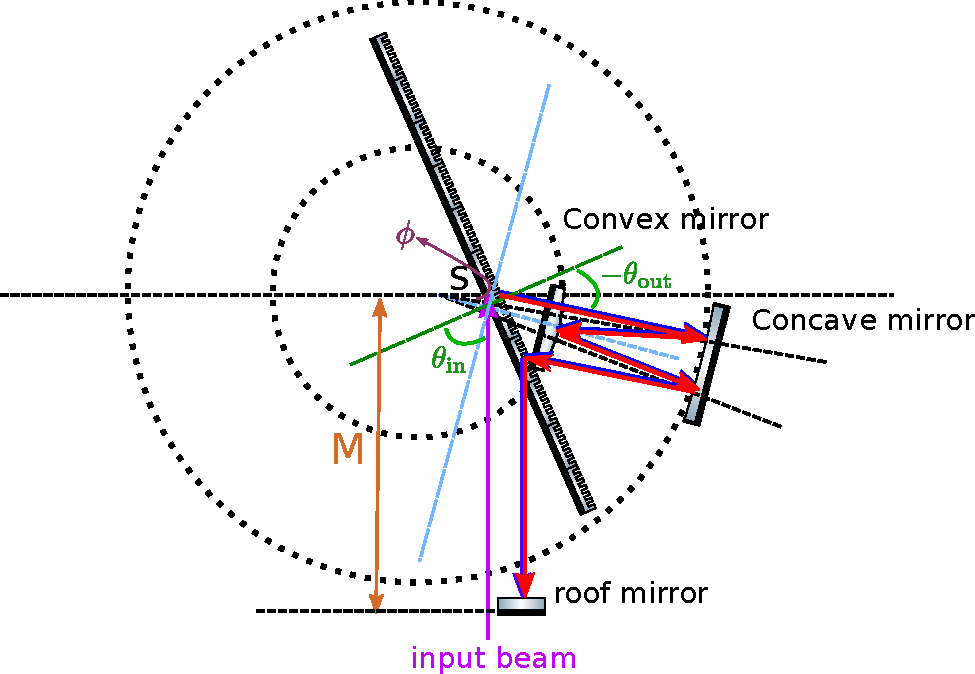
\includegraphics[width=\linewidth]{Offner stretcher (single grating).pdf}
\caption{Diagram of a single-grating transmissive Offner dechirper/stretcher.}
\label{fig:single_Offner_diagram}
\end{figure}

Suppose the deviation of the transmissive grating from the spherical center is $s$, and the convex and concave radius of curvature are $R$ and $2R$. From Fig.~\ref{fig:single_Offner_diagram} and \ref{fig:Offner_closed_view2}, we have
\begin{subequations}
\begin{align}
\Lambda\left(\sin\theta_{\text{out}}-\sin\theta_{\text{in}}\right) & =m\lambda \\
\frac{2R}{\sin(\theta_{\text{in}}-\theta_{\text{out}}-\frac{\pi}{2})} & =\frac{s}{\sin\theta}=\frac{\ell_1}{\sin\phi} \label{eq:Offner_eq2} \\
\frac{R}{\sin\theta} & =\frac{2R}{\sin\psi}=\frac{\ell_2}{\sin\left(\psi-\theta\right)} \label{eq:Offner_eq3} \\
\theta+\phi & =\theta_{\text{in}}-\theta_{\text{out}}-\frac{\pi}{2}. \label{eq:Offner_eq4} 
\end{align}
\end{subequations}

\begin{figure}[htbp]
\centering
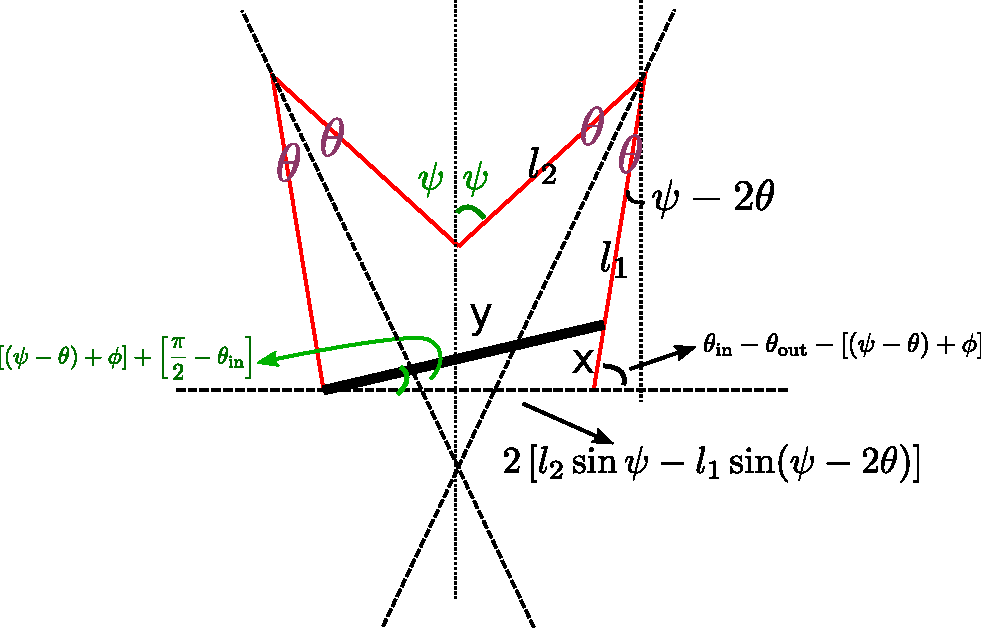
\includegraphics[width=.7\textwidth]{Offner_close_view2.pdf}
\caption{Diagram of an Offner dechirper/stretcher to calculate the propagation length.}
\label{fig:Offner_closed_view2}
\end{figure}

Note that if $\theta_{\text{in}}-\theta_{\text{out}}-\frac{\pi}{2}<0$, the diffracted beam goes to the upper-half plane, instead of going downward to the lower-half plane as in Fig.~\ref{fig:single_Offner_diagram}. Some angles may thus become negative.

To calculate $x$ (Fig.~\ref{fig:Offner_closed_view2}), we need the following relation,
\begin{subequations}
\begin{align}
\frac{2\left[\ell_2\sin\psi-\ell_1\sin(\psi-2\theta)\right]}{\sin(2\theta_{\text{in}}-\theta_{\text{out}}-\frac{\pi}{2}-2\left[\left(\psi-\theta\right)+\phi\right])} & =\frac{x}{\sin(\left[(\psi-\theta)+\phi\right]+(\frac{\pi}{2}-\theta_{\text{in}}))} \\
& =\frac{y}{\sin(\theta_{\text{in}}-\theta_{\text{out}}-\left[(\psi-\theta)+\phi\right])}.
\end{align}
\label{eq:Offner_xy}
\end{subequations}

If the deviation of the transmissive grating from the spherical center is small, different colors that go toward the roof mirror are almost parallel to the input beam. The total optical path length thus becomes
\begin{align}
\ell & = 2\left(\ell_1+\ell_2\right)-x+M-y\cos(\frac{\pi}{2}-\theta_{\text{in}}) \nonumber \\
& = 2\left(\ell_1+\ell_2\right)-x+M-y\sin\theta_{\text{in}} \nonumber \\
& \rightarrow 2\left(\ell_1+\ell_2\right)-x-y\sin\theta_{\text{in}},\quad \text{after ignoring }M.
\label{eq:Offner_l}
\end{align}

Here, we go through some algebra. Eq.~(\ref{eq:Offner_eq2}) leads to
\begin{equation}
\frac{2R}{-\cos(\theta_{\text{in}}-\theta_{\text{out}})}=\frac{s}{\sin\theta}=\frac{\ell_1}{\sin\phi}\quad\Rightarrow\quad\sin\theta=-\frac{s}{2R}\cos(\theta_{\text{in}}-\theta_{\text{out}})
\label{eq:Offner_theta}
\end{equation}
Eq.~(\ref{eq:Offner_eq4}) leads to
\begin{align}
\sin\phi = \sin(\theta_{\text{in}}-\theta_{\text{out}}-\frac{\pi}{2}-\theta) & =-\cos(\theta_{\text{in}}-\theta_{\text{out}}-\theta) \nonumber \\
& =-\cos(\theta_{\text{in}}-\theta_{\text{out}})\cos\theta-\sin(\theta_{\text{in}}-\theta_{\text{out}})\sin\theta.
\label{eq:Offner_phi}
\end{align}
With Eq.~(\ref{eq:Offner_phi}), Eq.~(\ref{eq:Offner_eq2}) leads to
\begin{align}
\ell_1 & =\frac{2R}{-\cos(\theta_{\text{in}}-\theta_{\text{out}})}\sin\phi \nonumber \\
& =2R\left[\cos\theta+\tan(\theta_{\text{in}}-\theta_{\text{out}})\sin\theta\right].
\end{align}
With Eq.~(\ref{eq:Offner_theta}), Eq.~(\ref{eq:Offner_eq3}) leads to
\begin{equation}
\sin\psi=2\sin\theta=-\frac{s}{R}\cos(\theta_{\text{in}}-\theta_{\text{out}}).
\label{eq:Offner_psi}
\end{equation}
With Eq.~(\ref{eq:Offner_psi}), Eq.~(\ref{eq:Offner_eq3}) leads to
\begin{align}
\ell_2 & =\frac{R}{\sin\theta}\sin(\psi-\theta) \nonumber \\
& =\frac{R}{\sin\theta}\left(\sin\psi\cos\theta-\cos\psi\sin\theta\right) \nonumber \\
& =\frac{R}{\sin\theta}\left(2\sin\theta\cos\theta-\cos\psi\sin\theta\right) \nonumber \\
& =R\left(2\cos\theta-\cos\psi\right).
\end{align}

To calculate $x$ and $y$, we use Eq.~(\ref{eq:Offner_theta}) to find $\left(\psi-\theta\right)+\phi$.
\begin{equation}
\left(\psi-\theta\right)+\phi=\left(\psi-2\theta\right)+\left(\theta_{\text{in}}-\theta_{\text{out}}-\frac{\pi}{2}\right).
\end{equation}
It is then put into Eq.~(\ref{eq:Offner_xy}).
\begin{align}
\frac{2\left[\ell_2\sin\psi-\ell_1\sin(\psi-2\theta)\right]}{-\cos(2\theta_{\text{in}}-\theta_{\text{out}}-2\left[\left(\psi-\theta\right)+\phi\right])} & =\frac{x}{\sin(\left(\psi-2\theta\right)-\theta_{\text{out}})}=\frac{y}{\sin(\frac{\pi}{2}-\left(\psi-2\theta\right))} \nonumber \\
\Rightarrow\quad\frac{2\left[\ell_2\sin\psi-\ell_1\sin(\psi-2\theta)\right]}{\cos(\theta_{\text{out}}-2\left(\psi-2\theta\right))} & =\frac{x}{\sin(\left(\psi-2\theta\right)-\theta_{\text{out}})}=\frac{y}{\cos(\psi-2\theta)}.
\end{align}
Finally, this leads to
\begin{subequations}
\begin{align}
& \begin{aligned}
x & =\frac{2\left[\ell_2\sin\psi-\ell_1\sin(\psi-2\theta)\right]}{\cos(\theta_{\text{out}}-2\left(\psi-2\theta\right))}\sin(\left(\psi-2\theta\right)-\theta_{\text{out}}) \\
& =\frac{2\left[\ell_2\sin\psi-\ell_1\sin(\psi-2\theta)\right]}{\cos(\psi-2\theta)\cot(\left(\psi-2\theta\right)-\theta_{\text{out}})-\sin(\psi-2\theta)}
\end{aligned} \\
& \begin{aligned}
y & =\frac{2\left[\ell_2\sin\psi-\ell_1\sin(\psi-2\theta)\right]}{\cos(\theta_{\text{out}}-2\left(\psi-2\theta\right))}\cos(\psi-2\theta) \\
& =\frac{2\left[\ell_2\sin\psi-\ell_1\sin(\psi-2\theta)\right]}{\cos(\left(\psi-2\theta\right)-\theta_{\text{out}})-\tan(\psi-2\theta)\sin(\left(\psi-2\theta\right)-\theta_{\text{out}})}
\end{aligned}.
\end{align}
\end{subequations}
With $\ell_1$, $\ell_2$, $x$, and $y$, we can calculate the optical path length $\ell$ [Eq.~(\ref{eq:Offner_l})].

Recall that the grating phase needs to be considered for a total accumulated phase. Unlike Treacy type, the blue light propagates farther than the red light (Fig.~\ref{fig:transmissive_Offner_grating_phase}). The larger the relative position $y$, the more grating phase needs to be added to redirect the light vertically. Thus, the single-pass total phase is
\begin{equation}
\phi_{\text{single-pass}}=k\ell-m\frac{y}{\Lambda}2\pi.
\end{equation}
The double-pass total phase is
\begin{equation}
\phi_{\text{double-pass}}=2\phi_{\text{single-pass}}=2k\ell-4m\pi\frac{y}{\Lambda}.
\end{equation}

\begin{figure}[htbp]
\centering
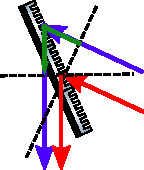
\includegraphics[width=0.2\linewidth]{transmissive Offner_grating phase.pdf}
\caption{The grating phase of an Offner-type transmissive grating dechirper/stertcher.}
\label{fig:transmissive_Offner_grating_phase}
\end{figure}

\subsection{Reflective single-grating Offner type}
Its optical path length is similar to the transmissive one except a reflective $\pi$ phase. The double-pass total phase is
\begin{equation}
\phi_{\text{double-pass}}=2k\ell+2\left(\pi-m\frac{y}{\Lambda}2\pi\right).
\end{equation}

\subsection{Aberration-free transmissive Offner type}
The Offner dechirper/stretcher discussed previously (Fig.~\ref{fig:single_Offner_diagram}) introduces an off-center distance to mitigate the difficulty of aligning two parallel gratings; however, this introduces aberration. Here, for broadband pulses, an aberration-free design (Fig.~\ref{fig:aberration-free-Offner}) is preferred to avoid distortion during the dechirping process.

\begin{figure}[htbp]
\centering
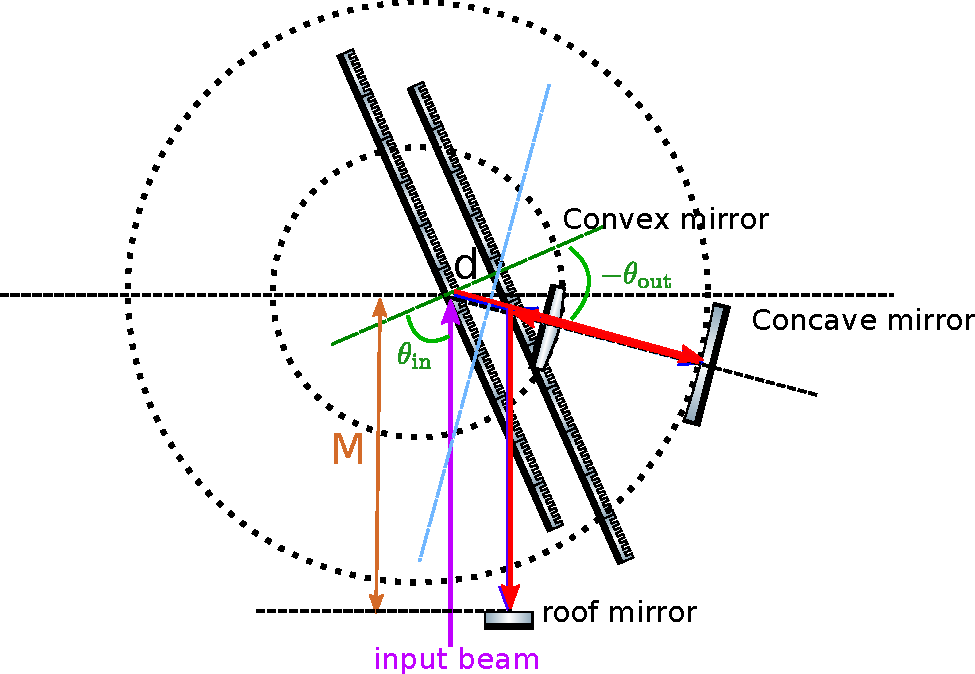
\includegraphics[width=\textwidth]{Offner stretcher (aberration-free double gratings).pdf}
\caption{Aberration-free double-grating transmissive Offner dechirper/stretcher.}
\label{fig:aberration-free-Offner}
\end{figure}

Assume the offset of two gratings is $d$, the path lengths to travel are, in order,
\begin{enumerate}
\item $\ell_1=2R$
\item $x=d\sec(-\theta_{\text{out}})\quad\Rightarrow\quad \ell_2=2R-x$
\item $\phi=-\theta_{\text{out}}-\left(\frac{\pi}{2}-\theta_{\text{in}}\right)\quad\Rightarrow\quad\ell_3=2\left(M-x\sin\phi\right)$
\item $\ell_2$
\item $\ell_1$
\end{enumerate}

The single-pass optical path length $\ell$ is
\begin{align}
\ell & =2\left(\ell_1+\ell_2\right)+\ell_3 \nonumber \\
& =8R-2x+2M-2x\sin\phi \nonumber \\
& \rightarrow-2x\left[1+\sin\phi\right]
\end{align}

Thus, the single-pass phase, including the grating phase, is
\begin{equation}
\phi_{\text{single-pass}}=k\ell-m\frac{d\tan(-\theta_{\text{out}})}{\Lambda}2\pi
\end{equation}
The double-pass total phase is
\begin{equation}
\phi_{\text{double-pass}}=2\phi_{\text{single-pass}}=2k\ell-4m\pi\frac{d\tan(-\theta_{\text{out}})}{\Lambda}.
\end{equation}

Fig.~\ref{fig:real_aberration-free-Offner} shows how a real Offner dechirper/stretcher is aligned.
\begin{figure}[!ht]
\centering
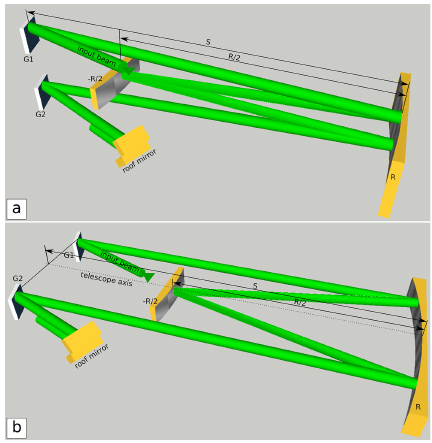
\includegraphics[width=.7\textwidth]{Offner_stretcher_real_design.png}
\caption{Two real configurations of an aberration-free double-grating Offner dechirper/stretcher \cite{Shvydkoy2020}.}
\label{fig:real_aberration-free-Offner}
\end{figure}

\clearpage

\printbibliography

\end{document}
